% IEEE TCSVT requires the IEEEtran class (Transactions Paper).  The previous
% article[10pt,twocolumn,letterpaper]+geometry layout rendered this manuscript at
% 16 pages; IEEEtran renders the identical body at 14 pages, which is exactly the
% TCSVT ceiling (see results/xtragpt/compile_20261002_r6/ECF_ieeetran_probe.pdf and
% the round-10 heartbeat entry).
\documentclass[journal,10pt]{IEEEtran}
\usepackage{times}
\usepackage{graphicx}
\usepackage{tikz}
\usetikzlibrary{arrows.meta,positioning}
\usepackage{amsmath,amssymb}
\usepackage{booktabs}
\usepackage{tabularx}
% dblfloatfix: corrects IEEEtran double-column figure* placement so that [b]
% (page-bottom) works for full-width floats, letting two full-width figures on the
% same page be split top/bottom instead of stacking back-to-back at the top.
\usepackage{dblfloatfix}
% Twocolumn: wide tables use table*+tabularx; in-column tables use
% tabularx{\columnwidth}; long display math uses aligned/split.
\newcolumntype{Y}{>{\raggedright\arraybackslash}X}
\usepackage{natbib}
\usepackage{xcolor}
\usepackage{hyperref}
\hypersetup{colorlinks=true,linkcolor=blue,citecolor=blue,urlcolor=blue}

% Figure-heavy manuscript: allow pages that are mostly floats so that full-width
% figure* environments are not deferred past the bibliography.
\setcounter{topnumber}{3}
\setcounter{dbltopnumber}{3}
\setcounter{totalnumber}{6}
\renewcommand{\topfraction}{0.95}
\renewcommand{\dbltopfraction}{0.95}
\renewcommand{\bottomfraction}{0.9}
\renewcommand{\textfraction}{0.05}
\renewcommand{\floatpagefraction}{0.7}
\renewcommand{\dblfloatpagefraction}{0.7}

% IEEEtran template convention: relax the penalty on page breaks inside displays.
\interdisplaylinepenalty=2500

% math_commands.tex — ECF paper
\newcommand{\Iou}{\ensuremath{\mathrm{IoU}}}
\newcommand{\gIou}{\ensuremath{\mathrm{gIoU}}}
\newcommand{\Rspa}{\ensuremath{R_{\mathrm{spa}}}}
\newcommand{\PrAt}[1]{\ensuremath{\mathrm{Pr@}#1}}
\newcommand{\Seg}{\texttt{[SEG]}}
\newcommand{\ECF}{\mathrm{ECF}}
\newcommand{\phih}{\ensuremath{\phi}}
\newcommand{\cR}{\ensuremath{\mathcal{R}}}
\DeclareMathOperator*{\argmax}{arg\,max}


\title{Ego-Corridor Fields:\\
Differentiable Corridor Rasterization\\
for Referring Rail Segmentation}
\author{Anonymous Authors}
\date{}

\begin{document}
\maketitle

\begin{abstract}
Referring expression segmentation (RES) couples a multimodal large language model with a frozen SAM2 decoder through a shared segmentation token.
In an ego-view rail frame, language already names the rail, so the task is to produce a corridor mask whose shape is more compactly described by parameters than by pixels.
Should that token state be decoded into a free-form SAM2 mask at all?
We replace the mask decoder with an Ego-Corridor Field (ECF): a small head maps the same token to 20 corridor parameters (centerline, width, vanishing point, topology) that a differentiable rasterizer turns into a mask, bypassing the SAM2 mask losses.
On FIRC2234 (208 original test frames, fp32), ECF-native decoding reaches 80.67 gIoU (97.6 and 87.98 precision at 0.5 and 0.7 IoU), outperforming same-protocol GroundingDINO+SAM2 (28.18) and Qwen2.5-VL-7B+SAM2 (25.60) by 2.9--3.2$\times$, and pretrained Sa2VA (14.32) by 5.6$\times$.
These three systems form the off-the-shelf reference set, the only comparison available for a benchmark introduced here.
ECF adds a $4.75$\,M-parameter head (0.205\% of the backbone) plus a $147.7$\,M LoRA adapter, and transfers eval-only to RailSem19-EgoPair (66.93) and RailBench 1L1R (54.21); its matched-training control (A1) collapses to 2.43 gIoU when SAM2 decodes the same state.
Code and evaluation scripts will be released at \url{https://github.com/lzdxwyh/ecf-corridor-fields} upon acceptance.
\end{abstract}

\begin{IEEEkeywords}
Referring expression segmentation, railway scene understanding, differentiable rasterization, multimodal large language model.
\end{IEEEkeywords}

\section{Introduction}
\label{sec:intro}

% Fig.1 前移到文件最顶（r12）：p1 装配期即声明 figure*[t]，LaTeX 顺延到 p2 页顶，
% 使 Fig.1 单独占 p2、Fig.2 teaser 留 p3。
\begin{figure*}[t]
\centering
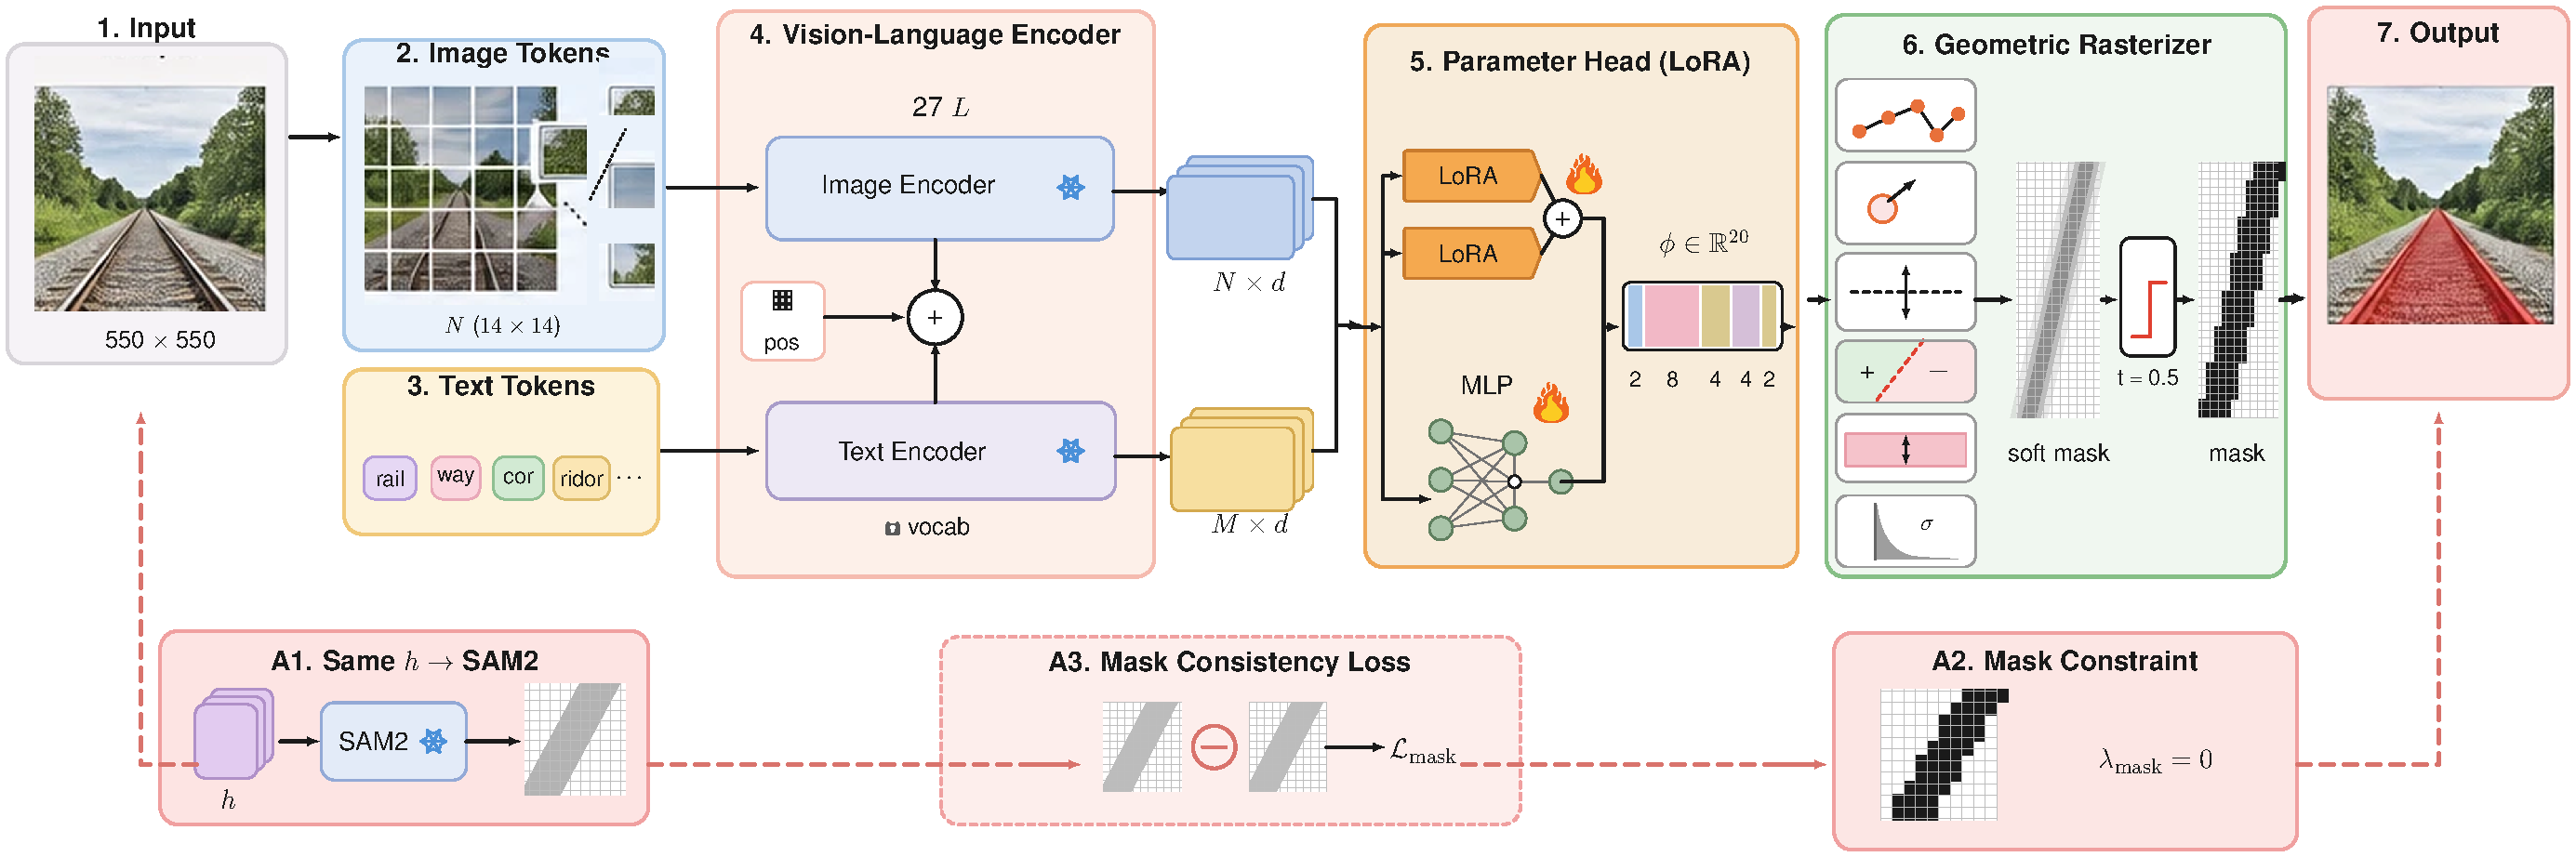
\includegraphics[width=\textwidth]{figures/ecf_framework_vec.pdf}%
\caption{The evaluated forward path, end to end. Panels~1--7: the $550{\times}550$ ego frame and the referring caption enter their token streams, and the frozen vision--language encoder processes both with the vocabulary left unchanged; the corridor head, trained through LoRA adapters on the frozen trunk, reads the first \Seg{} hidden state and emits the $20$ scalars of $\phih$ ($2|8|4|4|2$); the parameter-free rasterizer $\cR$ turns the field into a soft mask, and thresholding at $0.5$ yields the deployed mask. Bottom~row: the same state also reaches frozen SAM2, but its mask loss carries weight zero on this path, so mask supervision enters only through the corridor output (mask-consistency loss $\mathcal{L}_{\mathrm{mask}}$); decoding that state with SAM2 instead is the matched-training control A1 of Table~\ref{tab:ablate}.}
\label{fig:framework}
\end{figure*}

Rail infrastructure inspection relies on precisely localizing a \emph{specific} track among many, given a referring expression such as \emph{``near first from left rail track in frame''}.
This is a referring expression segmentation (RES) task \citep{yu2016refcoco,mao2016refcocog} in an ego-view, corridor-shaped setting: pixels pile up near the camera, thin out toward a vanishing point, and neighboring rails are near-duplicates under the caption.
Modern RES systems couple a multimodal large language model (MLLM) with a mask decoder; Sa2VA \citep{zhang2025sa2va} is the canonical design, where the MLLM emits a \Seg{} token whose hidden state is projected into a frozen SAM2 \citep{ravi2024sam2} decoder.
Off-the-shelf detector-plus-SAM2 pipelines fail badly on this task (gIoU ${\approx}$25--28), consistent with the known difficulty of grounding ordinal phrases like ``first from left'' with open-vocabulary detectors.

Two recent lines of work make the remaining design choice precise.
DeSa2VA \citep{dang2025desa2va} diagnoses three limitations of the shared \Seg{} interface---the token is semantically thin, SAM2 is never trained to read text, and a single hidden state cannot serve as a fine-grained visual prompt---and proposes an \emph{architectural} remedy: linear decoupling of MLLM hidden states, text-derived mask pre-training of SAM2, and mask-level self-feedback.
Independently, parametric lane estimators \citep{tabelini2021polylanenet,feng2022bezierlanenet} show that a corridor in a calibrated ego view is a low-dimensional object: a vanishing-point-anchored centerline plus a width field, not an arbitrary 2-D silhouette.
Rail-specific segmenters make a related simplification: RailSAM \citep{zhang2025railsam} and SMDE-YOLO \citep{lin2026smdeyolo} both produce \emph{class-level} rail masks, which certify that \emph{a} rail is present but do not decide \emph{which} rail an ordinal caption such as ``first from left'' names.
To our knowledge, neither line asks whether a Sa2VA-style \Seg{} token should stop talking to SAM2 altogether and instead emit that low-dimensional corridor, rasterized differentiably to a mask.

We ask that question.
After language has selected \emph{which} rail, the mask SAM2 is asked to produce is the region of a perspective corridor whose shape is more compactly described by parameters than by pixels, so our key idea is an Ego-Corridor Field ($\ECF$): the same \Seg{} hidden state is mapped by a ParamHead to $\phih \in \mathbb{R}^{20}$, and a differentiable rasterizer $\cR(\phih)$ produces the RES mask.
SAM2 remains in the codebase but is \emph{bypassed} on the training and inference path that we evaluate.
The rasterizer is part of the paradigm, not an optional post-process: if the same trained embeddings are fed to SAM2, the mask collapses (to $2.43$ gIoU), and if the raster mask loss is removed, the high-IoU rate drops sharply ($\PrAt{0.7}$ $87.98\to54.81$) while the mean falls only to $69.31$ gIoU.

Concretely, we train InternVL3-2B with LoRA and a 20-D ParamHead on the first \Seg{} token, using BCE+Dice on $\cR(\phih)$ against FIRC2234 masks plus a parameter loss on geometry-derived $\phih^{gt}$.
The training set is the original 1664 frames plus their horizontal flips (captions and $\phih^{gt}$ transformed to match the mirrored geometry), while val/test stay on original images; we evaluate only fp32 ECF-native decoding.
Our contributions are:

\begin{itemize}
\item \textbf{A carrier-level answer to DeSa2VA's sparse-\Seg{} diagnosis.} Without decoupling SAM2, we stop using SAM2 as the mask decoder and let \Seg{} predict a low-dimensional corridor parameterization.
\item \textbf{A differentiable rasterization closed loop.} $\cR$ maps $\phih$ to a soft mask; A1 (same weights, SAM2 decode) and A2 (no raster mask loss) are the falsifiers that show the loop is load-bearing.
\item \textbf{Same-protocol performance against the off-the-shelf reference set.} On FIRC2234 test (208 frames, fp32), ECF (gIoU 80.67) outperforms GroundingDINO+SAM2 (28.18) and Qwen2.5-VL-7B+SAM2 (25.60) by 2.9--3.2$\times$, and pretrained Sa2VA (14.32) by 5.6$\times$. These three off-the-shelf systems are the only reference rows of Table~\ref{tab:main}. The same checkpoint transfers, eval-only, to RailSem19-EgoPair and RailBench 1L1R. A SAM2 zero-shot oracle, reported in the supplementary material only, is not deployable and is not a competitor.
\end{itemize}

\paragraph{What is and is not compared.}
FIRC2234 is a new benchmark introduced here; to our knowledge, no published method has been trained on it, so the comparison is drawn against off-the-shelf systems applied without task-specific adaptation (Section~\ref{sec:setup}).
Those rows quantify how far an untrained generalist is from solving ordinal rail selection.
The control that isolates the carrier under matched training is A1 (Section~\ref{sec:ablate}): the very same ECF LoRA and ParamHead weights, decoded by SAM2 instead of $\cR$, fall to near-zero IoU, which counters the trivial reading that the masks come from the language backbone, and Section~\ref{sec:discussion} places this control next to DeSa2VA's encoder-side treatment.
Figure~\ref{fig:framework} is the evaluated forward path.

The rest of this paper is organized as follows.
Section~\ref{sec:related} positions the work against DeSa2VA, parametric lanes, and RES;
Section~\ref{sec:method} describes $\phih$, the ParamHead, and $\cR$;
Section~\ref{sec:exp} reports the protocol, the reference set, and the ablations;
Section~\ref{sec:discussion} discusses how a geometric carrier relates to token decoupling;
and Section~\ref{sec:conclusion} concludes.

% ---------------------------------------------------------------------------
% [FIGURE] ecf_teaser   spec: results/xtragpt/RELAYOUT_PLAN_and_FIGURE_SUITE.md Sec. 3.1 (F1)
% after the figure exists, replace this block with the rendered figure file figures/ecf_teaser_redraw.png
% ---------------------------------------------------------------------------
\begin{figure*}[t]
\centering
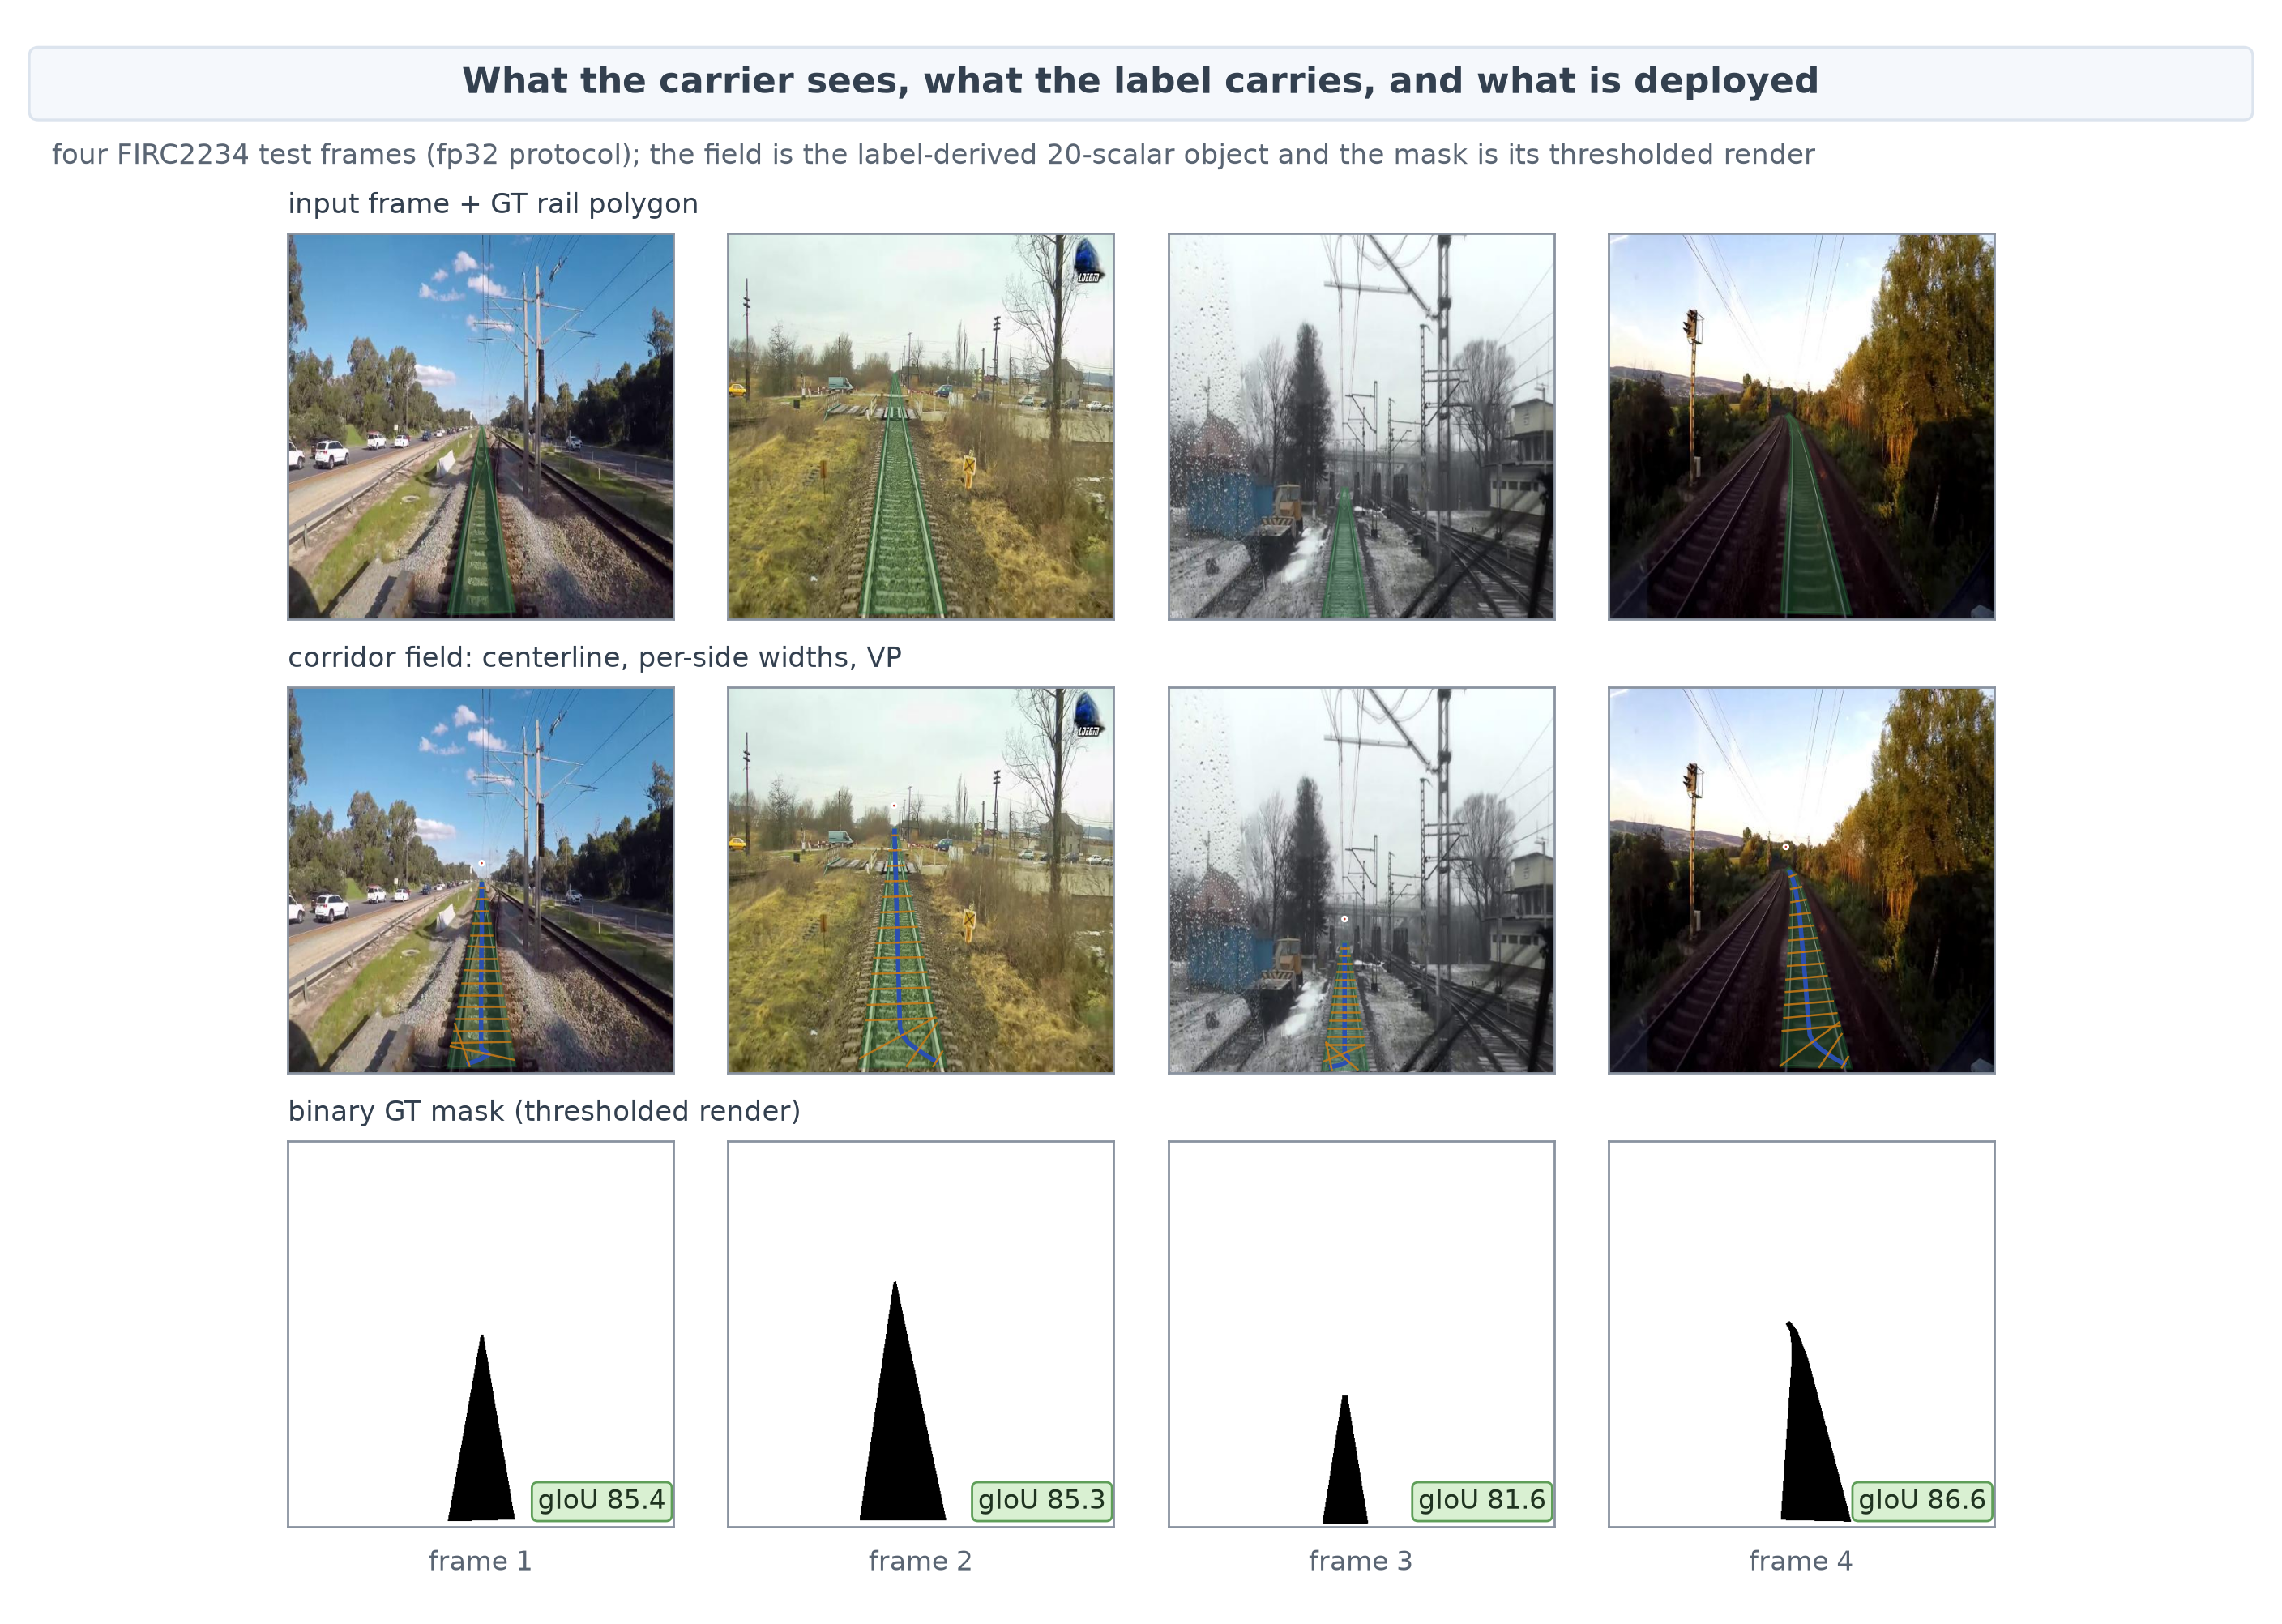
\includegraphics[width=\textwidth]{figures/ecf_teaser_redraw.png}
\caption{Capability of the corridor-field carrier on four ego-view rail settings. Each column shows the input frame, the predicted field overlaid as a centerline with a vanishing point, and the deployed binary mask; no mask on this path is decoded by SAM2.}
\label{fig:ph_ecf_teaser}
\end{figure*}

\begin{figure*}[t]
\centering
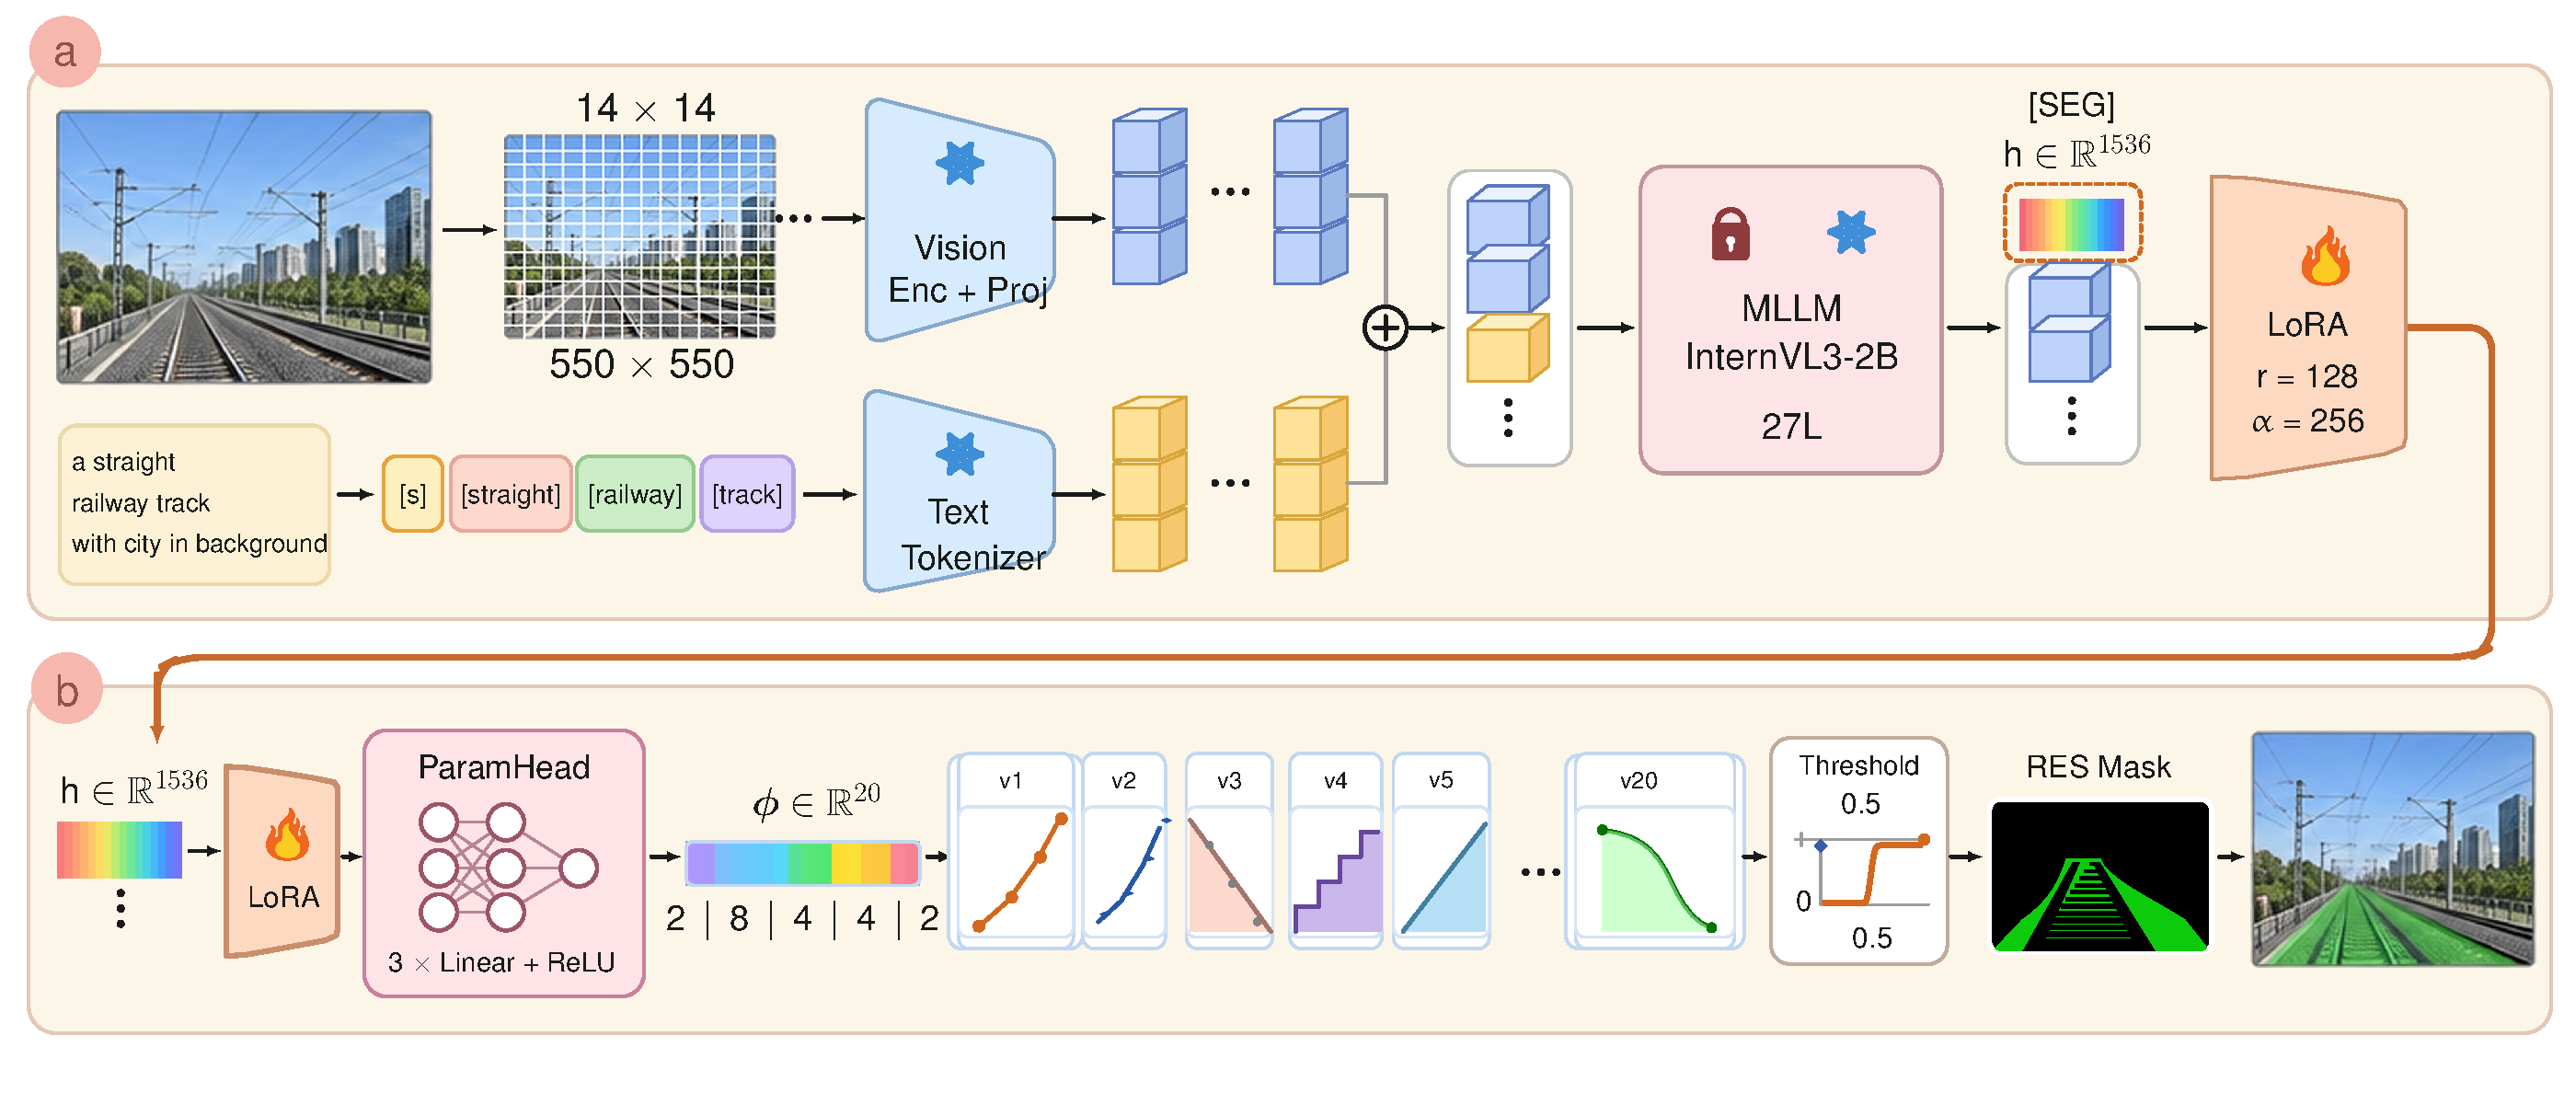
\includegraphics[width=\textwidth]{figures/ecf_forward_vec.pdf}%
\caption{Forward detail of the corridor head.
(a)~the referring frame through the frozen Sa2VA trunk (vision encoder and text tokenizer into the InternVL3-2B MLLM, whose first \Seg{} hidden state $h \in \mathbb{R}^{1536}$ is read by the LoRA-adapted head);
(b)~ParamHead (three linear layers with ReLU) maps $h$ to the corridor scalars $\phih$, which the differentiable rasterizer consumes slot by slot (vanishing point, $c_{1:K}$ centerline, left/right width samples, topology logits) to produce the soft mask and the thresholded RES mask.
Intended as a pictorial complement to Eq.~\eqref{eq:phi}: the slots are drawn as individual control curves to make the low-dimensional parameterization explicit.}
\label{fig:ecf_forward}
\end{figure*}

Figure~\ref{fig:ph_ecf_teaser} shows what the carrier produces across four ego-view rail settings, and Table~\ref{tab:quant} places it against the off-the-shelf reference set with the gIoU ratio to our row.


\begin{table}[t]
\centering
\small
\setlength{\tabcolsep}{4pt}
\caption{Accuracy and the gIoU ratio to our row (FIRC2234 test, fp32, $n{=}208$). Rows 2--4 are the off-the-shelf reference set of Table~\ref{tab:main}, measured by us on the same protocol; the ratio column gives our gIoU divided by the row's. A1 decodes the same trained $h$ with SAM2 (Table~\ref{tab:ablate}).}
\label{tab:quant}
\begin{tabularx}{\columnwidth}{@{}Ycc@{}}
\toprule
Method & \gIou & Ratio vs ours \\
\midrule
\textbf{Ours: ECF-native $\phih{\to}\cR$} & \textbf{80.67} & \textbf{$1.0\times$} \\
GroundingDINO+SAM2~\citep{liu2024groundingdino} & 28.18 & $2.9\times$ \\
Qwen2.5-VL-7B+SAM2~\citep{bai2025qwen2vl} & 25.60 & $3.2\times$ \\
Sa2VA pretrained~\citep{zhang2025sa2va} (no fine-tuning) & 14.32 & $5.6\times$ \\
A1: same $h$, SAM2 decode & 2.43 & -- \\
\bottomrule
\end{tabularx}
\end{table}

\section{Related Work}
\label{sec:related}

\paragraph{Referring expression segmentation and the \Seg{} interface.}
RES requires segmenting the object described by a natural-language expression, classically benchmarked on RefCOCO, RefCOCO+, and RefCOCOg \citep{yu2016refcoco,mao2016refcocog}.
The field has moved from proposal-matching pipelines to MLLM-based systems: LISA \citep{lai2024lisa} adds reasoning capability on top of SAM-style decoding, GLaMM \citep{rasheed2024glamm} unifies grounding with pixel-level generation, and Sa2VA \citep{zhang2025sa2va} marries LLaVA-class language models with SAM2 \citep{ravi2024sam2}, decoding \Seg{} tokens into masks through a frozen image encoder.
A parallel trend in generalist segmentation is to attach many task heads to a single foundation backbone: GLEE \citep{wu2024glee} unifies object-level tasks across images and videos, and SAM-Track \citep{cheng2023samtrack} chains SAM with a tracker for interactive video segmentation.
These systems keep a dense mask decoder as the carrier and vary what is fed into it; they supervise an arbitrary-shaped target as a dense mask.
The RES literature extends beyond dense decoding: PolyFormer predicts polygon vertices rather than pixels \citep{liu2023polyformer}, GRES extends the task to multi-target and no-target expressions with the region-based baseline ReLA \citep{liu2023gres}, and referring video object segmentation carries the caption-to-object interface to video \citep{miao2024htr}. PolyFormer is the closest parametric output, but its polygons come from a task-specific decoder, not from a referring token inside an MLLM.
We vary the carrier itself, for a target class whose shape is a \emph{perspective corridor}: in a calibrated ego view the referred rail is a vanishing-point-anchored centerline with a bilateral width field, and it is this low-dimensional structure, not a free silhouette, that the token is asked to emit.

DeSa2VA \citep{dang2025desa2va} is the closest architectural diagnosis of this interface, arguing that Sa2VA's shared \Seg{} token (i)~carries insufficient semantics, (ii)~is consumed by a SAM2 decoder that was never trained on text, and (iii)~provides only a sparse high-level hint rather than a fine-grained visual prompt.
The proposed remedy is linear decoupling of MLLM hidden states, a text-derived mask pre-training stage that turns labels into rasterized text masks for SAM2, and a one-step mask-reprompt loop.
On RefCOCO/+/g, its authors report that DeSa2VA-4B improves Sa2VA-4B by 3.7/6.1/5.1 points (82.6 / 77.8 / 79.2 versus 78.9 / 71.7 / 74.1), and their ablation additionally shows that \emph{text-derived mask pre-training of SAM2 without decoupling hurts} Sa2VA (RefCOCO 78.9$\to$73.4).
We keep the original Sa2VA token and do not add a decoupling module, and we make no claim that decoupling is unnecessary in general: our scope is targets whose shape is a perspective corridor, where the carrier can be parameterized directly.
What we change is what the token is allowed to mean---not a SAM2 prompt, but the parameters of a corridor field.
The two treatments act at different points of the same interface: DeSa2VA enriches the encoder-side prompt that SAM2 receives, and we replace SAM2 as the mask carrier; we read them as alternatives for different target classes rather than as a refutation.

\paragraph{Parametric lanes and differentiable rasterization.}
Ego-view lane and corridor estimation has long used low-dimensional models rather than free masks: polynomial or B\'ezier centerlines \citep{tabelini2021polylanenet,feng2022bezierlanenet}, perspective-aware transformers \citep{chen2022persformer}, cross-layer refinement \citep{zheng2022clrnet}, and conditional kernels that explicitly cover lane forks \citep{liu2021condlanenet}.
Those systems are detectors or segmenters with a geometric head; they are not MLLM referring models and they do not have to bind an ordinal caption to one of several parallel rails.
We import the geometric \emph{carrier} (a centerline plus bilateral width, carried alongside a vanishing-point slot) into a Sa2VA \Seg{} token.
The map from parameters to pixels is a differentiable rasterizer in the spirit of soft rendering \citep{kato2018renderer,liu2019softras}: occupancy is a sigmoid of signed distance to the polyline, so mask losses back-propagate into $\phih$.

\paragraph{Fine-grained special tokens.}
Momentor++ \citep{li2026momentorpp} shows that Video-LLM localization tokens only become useful after an intermediate grounded-processing stage; without it, discrete special tokens collapse into unrelated embeddings.
We do not implement temporal tokens; we borrow the observation that a special localization token is not by itself a complete spatial representation---for \Seg{}, DeSa2VA's sparse-prompt claim---and put the missing spatial detail into $\phih$ rather than into a second SAM2 stream.

\paragraph{Railway scene segmentation.}
Railway perception has its own segmentation literature, and it is the nearest neighbor of the task studied here.
RailSAM \citep{zhang2025railsam} keeps a frozen SAM encoder and injects domain geometry through multi-scale visual adapters in the mask decoder; its authors report that this parameter-efficient recipe significantly outperforms existing task-specific methods on RailSem19.
SMDE-YOLO \citep{lin2026smdeyolo} is the lightweight one-stage counterpart: Scharr-based edge enhancement, a dynamic multi-branch feature pyramid, and a decoupled segmentation head; its authors report $2.59$\,M parameters and $58.7$ FPS at $640{\times}640$ on a rail instance-segmentation benchmark.
Both solve \emph{class-level} rail segmentation, where every rail pixel is a valid ``rail'', whereas we solve expression-level target \emph{selection}: given an ordinal caption, exactly one rail is correct, and a class-level mask is a failure.
The two problems are orthogonal.
RailSAM is also a direct PEFT precedent for this paper: it shows that adapters can inject domain geometry into a generalist decoder, while ECF shows that the \Seg{} token of a referring model can emit that geometry directly instead.

\paragraph{Rail and ego-view referring scenes.}
Ego-view rail perception is a distinct regime: targets are corridor-shaped, captions are near-duplicates, and perspective creates severe pixel imbalance.
RailSem19 \citep{zendel2019railsem19} provides semantic rail-scene labels and reports rail mIoU in the 55--75 range for classical segmentation models, while detection+SAM2 pipelines built on open-vocabulary detectors \citep{liu2024groundingdino,bai2025qwen2vl} struggle with ordinal referring expressions (gIoU ${\approx}$25--28, Section~\ref{sec:exp}).
Our benchmark, FIRC2234, is a single-rail referring-segmentation corridor set with 1664/208/208 original-image splits (Figure~\ref{fig:dataset}(a)); training uses the original frames and their horizontal flips (Section~\ref{sec:data}), and two additional fill-band sets (RailSem19-EgoPair and RailBench 1L1R) are eval-only and are never mixed into the FIRC main table.


\section{Method}
\label{sec:method}

The section follows the path of a single frame. Section~\ref{sec:task} fixes the task and the token that is read, Section~\ref{sec:phi} defines the twenty scalars that stand in for the mask, Section~\ref{sec:rast} renders those scalars into pixels with a fixed differentiable rasterizer, and Section~\ref{sec:train} states what is trained and under which losses. The model still outputs a mask, but the object it predicts is a corridor field, and that separation drives each of the choices below.

\subsection{Task and frozen Sa2VA token}
\label{sec:task}

We consider referring expression segmentation (RES): given an image $I$ of height $H$ and width $W$ and a referring caption $C$, the model must output a binary mask of the referred object.
We build on the \emph{undecoupled} Sa2VA architecture \citep{zhang2025sa2va}: an InternVL3-2B MLLM emits a \Seg{} token whose hidden state $h \in \mathbb{R}^{1536}$ would normally be projected into a frozen SAM2 \citep{ravi2024sam2} decoder.
Unlike DeSa2VA \citep{dang2025desa2va}, we do not split $h$ into text and visual streams, and we do not teach SAM2 to read labels.
On the path we evaluate, SAM2 mask decoding is bypassed---$h$ is consumed only by the corridor head below---and we do \emph{not} add a dedicated corridor token, since an extra vocabulary item would require a new, untrained embedding; ParamHead instead reads the first \Seg{} hidden state (training and fp32 eval).

The output space is the first commitment. A dense carrier spends $H{\times}W$ binary decisions per frame and leaves the structure of the target implicit, whereas a corridor is fixed by a few geometric quantities. The question a mask decoder answers jointly is therefore split in two. Which rail the caption names is a language problem, and which region that rail occupies has, for a perspective corridor, a known low-dimensional form. ECF keeps the first on the MLLM and answers the second with an explicit parametric carrier, so the token no longer encodes a silhouette pixel by pixel. A1 isolates this choice by decoding the same trained state with SAM2.

Three properties of the interface decide how the head is wired. The \Seg{} token is emitted in the same autoregressive pass that writes the referring completion, so its hidden state is conditioned on the caption tokens that precede it, and an ordinal phrase such as ``first from left'' reaches the mask through that state rather than through a second text encoder. A generation may contain more than one \Seg{} token, and we read the first in training and in evaluation. The vocabulary is left untouched. A dedicated corridor token would add an embedding row with no pretraining support and would ask a fresh vector to carry what the existing \Seg{} row already carries.

\textbf{Scope.} The carrier describes one corridor with one centerline, which holds for every frame of FIRC2234 and for both transfer sets of Section~\ref{sec:transfer}. It does not require a calibrated camera. The vanishing point is a free coordinate of $\phih$, not a projection of a known optical axis, so the parameterization applies to any ego view in which rails converge. Targets without a dominant axis, a crowd or a piece of equipment, fall outside this scope.

% Fig.4（pipeline）改 [t] 并前移到 §Method 开头（r12）：Fig.3 已占 p4 页顶，
% 此块在 p4 装配期声明 -> 顺延到 p5 页顶，与 Fig.3 分页；Fig.5（rast）仍为 [b]。
\begin{figure*}[t]
\centering
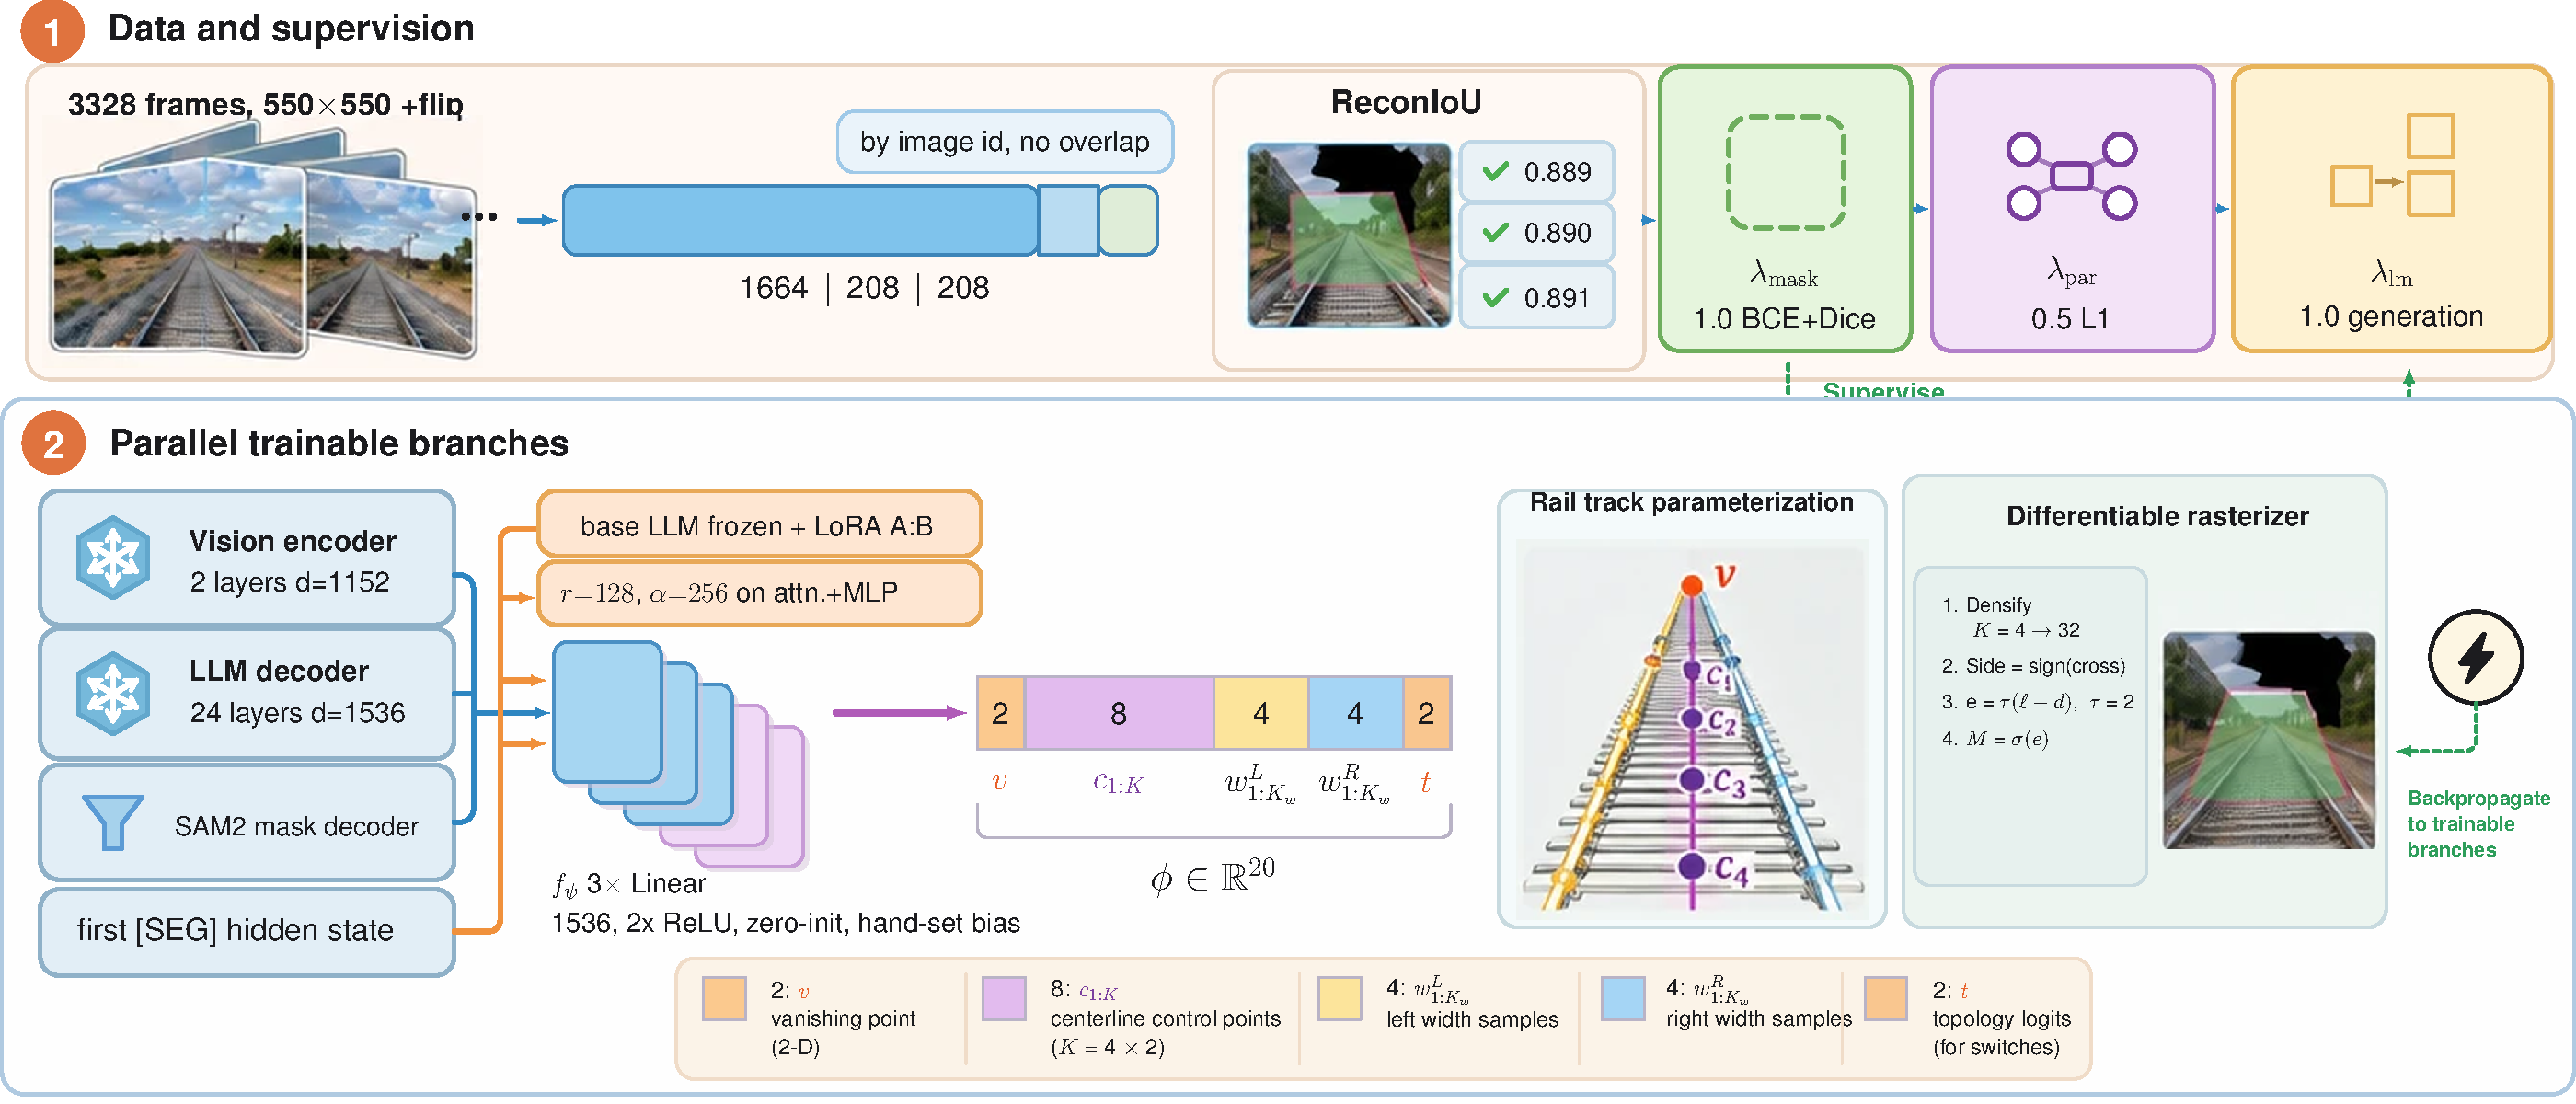
\includegraphics[width=\textwidth]{figures/ecf_pipeline_vec.pdf}%
\caption{Data, supervision, and the trainable branches. Band~1: the $3328$-frame corpus ($550{\times}550$, original$\cup$hflip) with the $1664|208|208$ split by image id, the per-split ReconIoU of the reconstructed labels ($0.889/0.890/0.891$), and the three primary loss weights of the recipe ($\lambda_{\mathrm{mask}}{=}1.0$ BCE${+}$Dice, $\lambda_{\mathrm{par}}{=}0.5$ L1, $\lambda_{\mathrm{lm}}{=}1.0$ generation). Band~2: the frozen trunk (vision encoder, LLM decoder, SAM2 mask decoder) carries LoRA ($r{=}128$, $\alpha{=}256$ on the LLM attention and MLP projections) and the ParamHead (three linear layers, zero-initialized, hand-set bias); the $20$ scalars of $\phih$ (legend: $2$ vanishing point, $8$ centerline, $4{+}4$ widths, $2$ topology) enter the differentiable rasterizer (densify $K{=}4$ to $32$, side sign, margin at $\tau{=}2$, $M{=}\sigma(e)$), and the dashed arrows mark the gradient that returns to the trainable branches.}
\label{fig:ecf_pipeline}
\end{figure*}

\subsection{Ego-Corridor Field}
\label{sec:phi}

The target in an ego-view rail frame is a perspective corridor, which we represent by a low-dimensional corridor field
\begin{equation}
\begin{aligned}
\phih
&= \big(
\mathbf{v},\;
\mathbf{c}_{1:K},\;
\mathbf{w}^{L}_{1:K_w},\;
\mathbf{w}^{R}_{1:K_w},\;
\mathbf{t}
\big) \\
&\in \mathbb{R}^{20},
\end{aligned}
\label{eq:phi}
\end{equation}
with $K{=}4$ centerline control points ($8$ coordinates), $K_w{=}4$ left/right width samples, a 2-D vanishing point $\mathbf{v}$, and $2$ topology logits $\mathbf{t}$ reserved for forks.
Centerline and vanishing-point coordinates live in image-normalized $[0,1]$, and widths are positive fractions of the image short side; a Rail-Path Verifier on $\mathbf{t}$ is \emph{not} trained, and we do not claim fork disambiguation.

The twenty scalars are budgeted by what the geometry has to bend. Four centerline points carry one inflection, which covers the straight, the gently curving and the strongly curving frames of the benchmark, and four width samples per side let the near field widen without forcing the far field to do the same. The remaining four slots are the anchor and the topology. The carrier compresses a $550{\times}550$ mask by about four orders of magnitude, and Section~\ref{sec:train} measures what survives.

Every coordinate is image-normalized, so the field does not depend on the resolution at which it is rendered, and every width is a fraction of the short side, so the same $\phih$ stays meaningful when the aspect ratio changes. The horizontal flip used in training is a closed-form involution on the parameters. The horizontal coordinate of each control point and of the vanishing point maps to one minus itself, the left and right width slots exchange roles, and the two topology logits exchange order. The flipped training copies are therefore exact.

A lightweight ParamHead $f_\psi$ maps $h$ to $\phih$: three linear layers with ReLU, last-layer weights zero-initialized, and a hand-set bias (vanishing point near $(0.5,0.2)$, centerline along the image axis, widths ${\approx}0.08$).
With zero initial weights it therefore starts as a plausible corridor rather than a random mask, as Figure~\ref{fig:ecf_forward} shows in detail: the \Seg{} hidden state through ParamHead to the corridor scalars and on to the per-slot curves the rasterizer consumes.
There is no output sigmoid or softplus: range constraints are applied inside the rasterizer (centerline clamped to $[0,1]$, widths $\ge 10^{-4}$).

The initialization is a prior rather than a random start. With the last layer at zero the head returns its bias at step zero, and that bias already describes a corridor running up the image axis. The first mask loss is therefore evaluated on a plausible corridor, and the gradient reaching $f_\psi$ corrects a shape instead of searching for one. The head is kept small on purpose, with $4.75$\,M parameters against a $2316.2$\,M frozen backbone, so the capacity for the task sits in the LoRA-adapted language model.

\subsection{Differentiable rasterization}
\label{sec:rast}

The differentiable rasterizer $\cR$ turns $\phih$ into a soft mask $M \in (0,1)^{H \times W}$: control points are scaled to pixels and densified along the polyline, and for each pixel a distance $d$ to the polyline is compared to a side-dependent width $\ell$ (mean left width if the signed offset is positive, mean right width otherwise):
\begin{equation}
\begin{aligned}
M &= \sigma\!\big(\tau\,(\ell - d)\big), \\
\hat{M} &= [M \ge 0.5],
\end{aligned}
\label{eq:rast}
\end{equation}
with temperature $\tau{=}2$; we call $e{=}\tau(\ell-d)$ the margin; Figure~\ref{fig:ecf_rast} expands the rasterizer one operation at a time.

Two operations sit between the scalars and the sigmoid. Densification joins the four control points into a polyline and resamples it to thirty-two points, so the distance field sees a curve rather than four vertices and the far field, where consecutive control points are far apart in pixels, does not develop polygonal corners. The distance $d$ of a pixel is then the minimum point-to-segment distance over the thirty-two segments, and the signed offset is measured along the left normal of the nearest segment. Only the sign of that offset is used, because the width on each side enters as a single scalar.

The margin is the only quantity the sigmoid sees, and it is what carries the gradient from the mask back to the parameters. The distance $d$ is Lipschitz in pixel position with constant one, the width $\ell$ is linear in the width slots, and $\sigma$ is smooth, so $\partial M/\partial \phih$ exists away from the centerline, where the side switches and the width jumps if the two sides differ, and away from the set where two segments are equidistant. Both sets are measure zero, and the jumps inside $\cR$ do not block the mask loss from reaching $f_\psi$. The temperature fixes the width of the soft band. At $\tau{=}2$ the ten to ninety percent transition spans about $2.2$ pixels at $550{\times}550$, narrow enough that the soft mask and the thresholded mask agree almost everywhere, and wide enough that a pixel just outside the boundary still receives a gradient.

The corridor $\cR$ renders is therefore a constant-width capsule around the polyline: the $K_w$ width samples enter only through their per-side mean, so a width profile \emph{along} the corridor is not currently modeled and the $\mathbf{w}^{L},\mathbf{w}^{R}$ slots act as a low-dimensional width control rather than as a dense envelope.
The vanishing point $\mathbf{v}$ is part of $\phih$ and is supervised in the parameter loss; occupancy itself is a distance-to-polyline field, not a ray-cast from $\mathbf{v}$.
Because $\sigma$ is smooth, mask losses back-propagate into $f_\psi$ and into the LoRA that produces $h$.
Figure~\ref{fig:framework} renders the evaluated forward path end to end, Figure~\ref{fig:ecf_forward} details the ParamHead mapping from $h$ to the corridor scalars, Figure~\ref{fig:ecf_pipeline} shows how the training signal is assembled and split across the trainable branches, and Figure~\ref{fig:ecf_rast} records where each step's gradient comes from.

\subsection{Training}
\label{sec:train}

Let $M^{gt}$ be the rasterized ground-truth rail mask and $\phih^{gt}$ a geometry-derived label (offline mask$\to$centerline/width/vanishing-point; train/val/test median ReconIoU $0.889/0.890/0.891$, supplementary material, Section~D).
Figure~\ref{fig:ecf_pipeline} lays out this recipe: the $3328$-frame corpus with its $1664|208|208$ split, the three loss weights, and the trainable branches that the gradient reaches.

The label is derived once, offline, from the annotation polygon. The polygon is rasterized, its medial axis gives an ordered centerline from the near field to the far field, and the width on each side is read by casting rays normal to the centerline until they leave the mask. The vanishing point comes from the two boundary lines of the corridor, and the topology logits come from the branch structure of the skeleton, which is trivial on single-rail frames. The procedure is deterministic and consumes only the released masks, so the parameter supervision adds no annotation cost.

The check on that label is reconstruction IoU. We render $\phih^{gt}$ with a non-learned reference renderer and compare the result to the original mask under the same IoU used for evaluation. The median is $0.889$ on train, $0.890$ on val and $0.891$ on test, so a twenty-dimensional corridor reproduces about nine tenths of the annotated region. The remaining tenth is the part of the annotation that the parameterization does not carry, so the figure bounds the label rather than the trained decoder.

The primary loss is
\begin{equation}
\begin{aligned}
\mathcal{L}
&= \lambda_{\mathrm{mask}}\mathcal{L}_{\mathrm{mask}}(\cR(\phih), M^{gt}) \\
&\quad + \lambda_{\mathrm{par}}\mathcal{L}_{\mathrm{param}}(\phih, \phih^{gt}) \\
&\quad + \lambda_{\mathrm{lm}}\mathcal{L}_{\mathrm{LM}},
\end{aligned}
\label{eq:loss}
\end{equation}
with $\lambda_{\mathrm{mask}}{=}1.0$, $\lambda_{\mathrm{par}}{=}0.5$, and $\lambda_{\mathrm{lm}}{=}1.0$ (generation); $\mathcal{L}_{\mathrm{param}}$ is an L1 on the non-topology coordinates, and $\mathcal{L}_{\mathrm{mask}}$ a sum of BCE and Dice on the soft raster, with SAM2 mask/dice losses replaced by a finite zero on this path (supplementary material, Section~F).

The reported training recipe also includes a weak width-monotonicity term ($0.1$), a far-row mask weight ($\gamma{=}1.0$), and small auxiliary weights on the topology logits and the frozen Verifier head (supplementary material); we do \emph{not} claim these as contributions---a later physics-heavy recipe failed to help far-field IoU and is not a main-table variant.

\textbf{Optimization.} LoRA ($r{=}128$, $\alpha{=}256$) on the LLM's attention and MLP projections, with the vision encoder frozen and ParamHead trainable, under AdamW at learning rate $4{\times}10^{-5}$ with mixed-precision fp16 and gradient clipping at $0.5$.
The reported checkpoint is a single $133{,}120$-iteration schedule on orig$\cup$hflip (3328 frames, 10 repeats, 4 epochs), initialized from the official InternVL3-2B Sa2VA weights (supplementary material, Section~F).

\textbf{Inference.} Generate the referring completion, take the first \Seg{} hidden state, $f_\psi \to \cR \to$ threshold $0.5$, all in \textbf{fp32}; fp16 evaluation is never used, since in our runs it collapses \Seg{} decoding.
The decode is one head application and one rasterization, with no mask prompt loop and no autoregressive repair, so a frame cannot depend on the mask predicted for another frame.
Figure~\ref{fig:framework} summarizes this evaluated forward path end to end.

% Fig.4 的浮动块放在 Training 小节之后，使它与 Fig.3 之间隔有实质正文，
% 避免两张全宽流程图在同一页背靠背堆叠（LaTeX 对相邻 figure*[t] 会连续堆到同一页顶）。
% Fig.5（rast）改用 [b]（页底，需 main.tex 的 dblfloatfix）：Fig.3 前移后它曾与
% Fig.6（dataset）同落一页且仅隔图注 → 改页底后可与之分居页顶/页底。
\begin{figure*}[b]
\centering
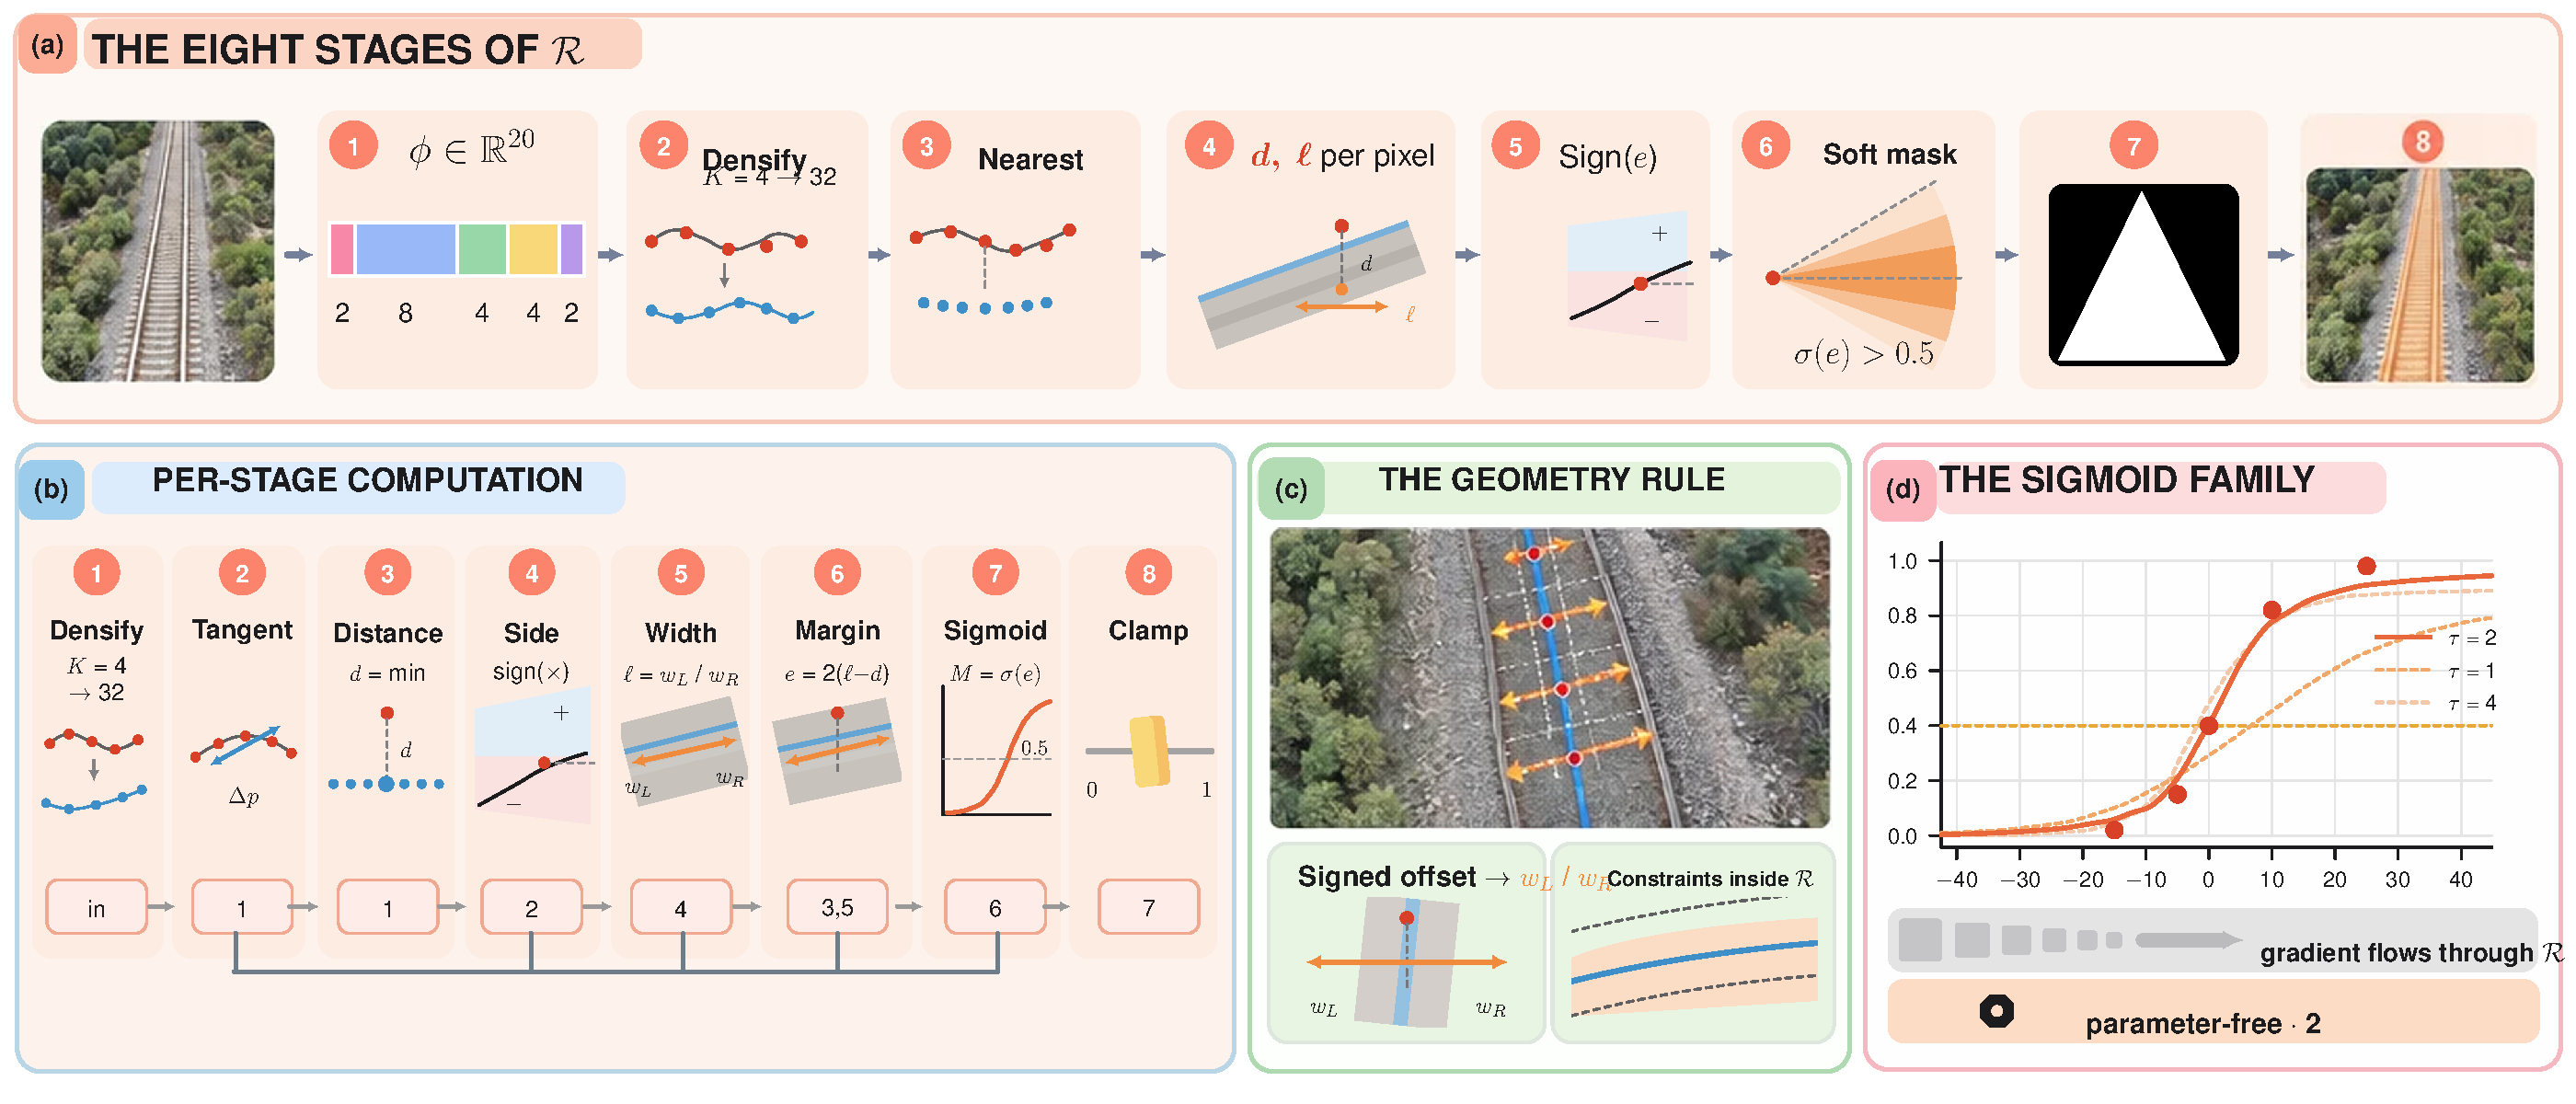
\includegraphics[width=\textwidth]{figures/ecf_rasterizer_vec.pdf}%
\caption{The differentiable rasterizer, operation by operation, on a test frame.
(a)~the eight stages that turn $\phih$ into the deployed mask, from the $20$ scalars through densification to the thresholded mask.
(b)~the same stages as explicit computations with their dependency badges: stage~$1$ is the only fan-out point and stage~$6$ the only two-input merge, so the chain stays strictly serial apart from the margin $e{=}\tau(\ell-d)$ at $\tau{=}2$.
(c)~the geometry rule on a test frame: the signed offset selects the left or right width, and the range constraints are applied inside $\cR$.
(d)~the $\sigma$ family for the temperatures the rasterizer admits; every member is smooth, so the mask loss crosses $\cR$ into $f_\psi$ and on into the LoRA, and the rasterizer itself holds no parameters.
The mask-production stage costs $2.90$\,ms of rasterization plus $2.30$\,ms of head evaluation, i.e.\ $2.42\%$ of the $214.6$\,ms end-to-end latency.}
\label{fig:ecf_rast}
\end{figure*}

\section{Experiments}
\label{sec:exp}

\subsection{Dataset}
\label{sec:data}

FIRC2234 is a single-rail referring-segmentation corridor set of ego-view rail frames, all $550{\times}550$ pixels, split by original image ID into 1664/208/208 train/val/test frames with no overlap.
Every frame contains exactly one rail polygon and carries an ordinal caption; the val and test splits use a single caption string each (``near first from left rail track in frame''), and the train split contains two distinct strings across 1664 frames.
The referred rail occupies a median $4.7\%$ of the image (p10--p90 $3.2$--$7.3\%$ on test), i.e.\ a thin perspective corridor rather than a compact object, precisely the regime in which a dense, arbitrary-shaped mask decoder is a poor carrier.
Table~\ref{tab:data} summarizes the protocol, and Figure~\ref{fig:dataset} shows both the resulting distributions and six sample frames.
Training uses the 1664 original frames \emph{and} their horizontal flips (3328 frames): images, masks, and $\phih^{gt}$ are mirrored and the caption's spatial words are swapped accordingly, while photometric jitter is online and does not write extra files.
Val and test remain the original 208+208 images and captions, all numbers below that are not marked as transfer are computed on this 208-frame test split, and all evaluation is fp32.

\begin{figure*}[t]
\centering
\IfFileExists{figures/fig2_firc_dataset.pdf}{%
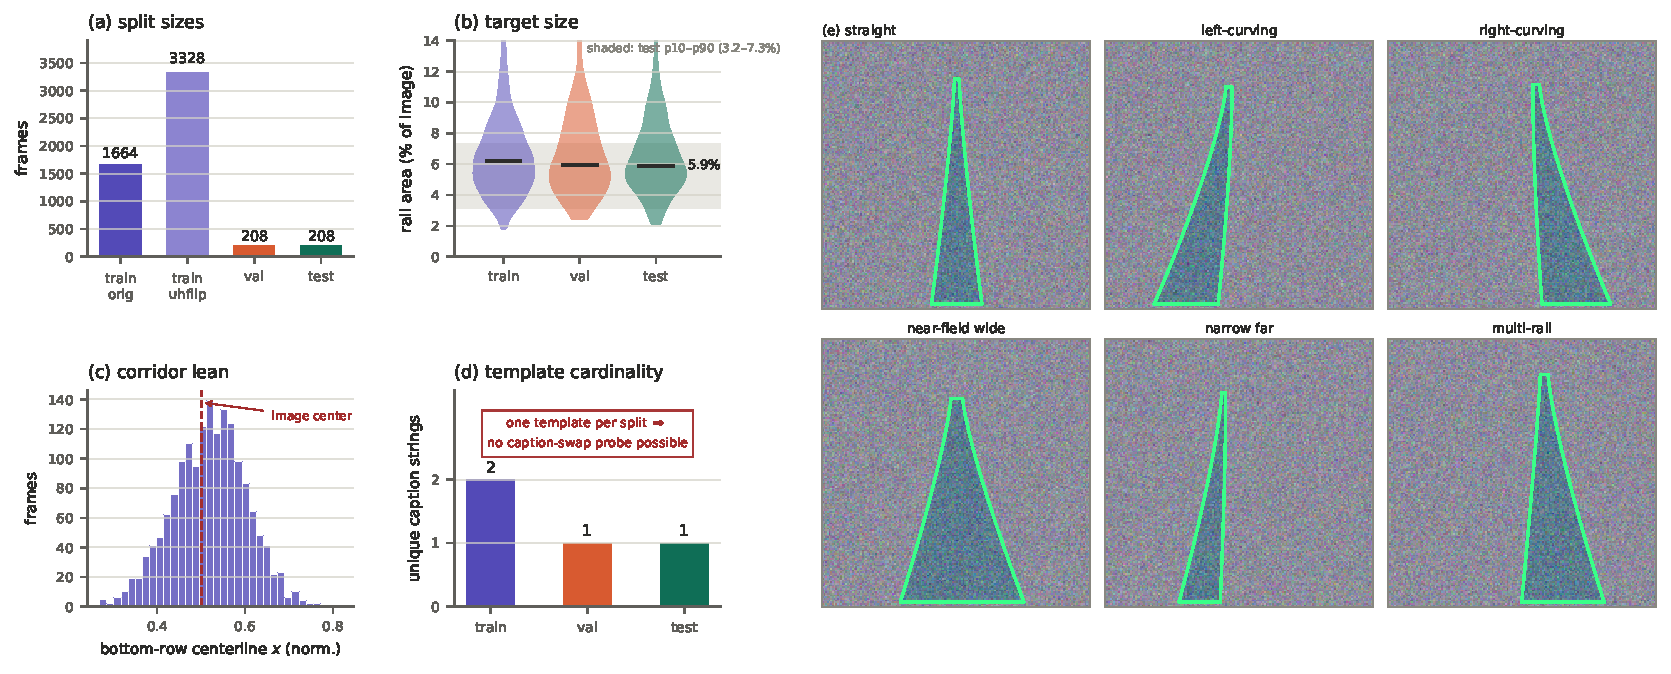
\includegraphics[width=\textwidth]{figures/fig2_firc_dataset.pdf}%
}{%
\fbox{\parbox{0.95\textwidth}{\centering\vspace{14mm}Dataset panel omitted in this build.\vspace{14mm}}}%
}%
\caption{FIRC2234 at a glance.
(a)~split sizes, including the $\times2$ horizontal-flip doubling that the train split receives.
(b)~the rail-area distribution per split, the mask-to-image ratio whose p10--p90 range on test ($3.2$--$7.3\%$) is the thin-corridor regime the carrier is designed for.
(c)~the horizontal position of the corridor centerline on the bottom image row, a proxy for how far the corridor leans out of the image axis: the spread is what a $20$-D carrier must cover.
(d)~the number of distinct caption strings per split; a single eval template is why no caption-swap linguistic probe can be run on this dataset (Section~\ref{sec:transfer}).
(e)~six test-style frames spanning the split, with the ground-truth rail polygon in green; from left to right, top to bottom: straight, left-curving, right-curving, the widest near-field frame, a narrow far-field corridor, and a multi-rail ordinal frame.
Panels (a)--(d) are computed from the released annotations; panel (e) is rendered from the annotation geometry.}
\label{fig:dataset}
\end{figure*}

\begin{table}[t]
\centering
\small
\setlength{\tabcolsep}{4pt}
\caption{FIRC2234 protocol. All frames are $550{\times}550$; statistics are computed from the released annotations. Rail area is the mask-to-image ratio (test p10--p90 $3.2$--$7.3\%$). Val and test each use one caption string; the train split uses two.}
\label{tab:data}
\begin{tabularx}{\columnwidth}{@{}lYcc@{}}
\toprule
Split & Role & Frames & Rail area (med.) \\
\midrule
train & orig $\cup$ hflip & 1664 ($\times2$) & $4.7\%$ \\
val & eval & 208 & $4.7\%$ \\
test & eval & 208 & $4.7\%$ \\
\bottomrule
\end{tabularx}
\end{table}

\subsection{Setup}
\label{sec:setup}

\textbf{The reference set.}
FIRC2234 is introduced in this work; consequently, to our knowledge, \emph{no previously published method has been trained on it}.
The comparison set therefore consists of the strongest \emph{off-the-shelf} systems that apply to ego-view rail frames without task-specific adaptation---the same set a practitioner faces at deployment time.
We report gIoU (mean per-frame mask IoU), \PrAt{0.5} and \PrAt{0.7} (the share of frames with IoU ${\ge}0.5$ and ${\ge}0.7$), and SegRate (fraction of frames with any predicted mask).
The reference rows are all off-the-shelf, measured by us on the same protocol: (i)~pretrained Sa2VA \citep{zhang2025sa2va} with no fine-tuning; (ii)~GroundingDINO-base \citep{liu2024groundingdino} detecting ``rail'' $\rightarrow$ leftmost box $\rightarrow$ SAM2 \citep{ravi2024sam2} mask; (iii)~Qwen2.5-VL-7B \citep{bai2025qwen2vl} grounding $\rightarrow$ leftmost box $\rightarrow$ SAM2 mask; and (iv)~a SAM2 zero-shot \emph{oracle} that auto-segments an $8{\times}8$ point grid and picks, per image, the best mask among 192 candidates against ground truth, which has \emph{no target-selection mechanism} and is not deployable---we report it in the supplementary material only as a probe of what the frozen-SAM2 segmenter can yield on its own, not as a reference row.
Rows (i)--(iii) receive no gradient update on FIRC, whereas our row is trained with LoRA$+$ParamHead on original$\cup$hflip under the same evaluation protocol; DeSa2VA \citep{dang2025desa2va} is discussed as mechanistic related work (Section~\ref{sec:discussion}, supplementary material, Section~A), not as a same-protocol FIRC reference row.

\textbf{Decoder cost.}
The advantage ECF claims is architectural, and so is its cost signature: on the evaluated path the SAM2 image encoder and dense mask decoder are removed from inference, and the only learned module between the \Seg{} hidden state and pixels is a three-layer head producing a 20-D $\phih$ consumed by a fixed differentiable rasterizer.
We profile that path directly (fp32, batch $1$, $550{\times}550$, one A100-class GPU) and report the measurement rather than an architectural estimate.
The ParamHead holds $4.75$\,M parameters, i.e.\ $0.205\%$ of the $2316.2$\,M-parameter backbone, and the LoRA adapter adds $147.7$\,M.
End-to-end ECF-native inference averages $214.6 \pm 14.2$\,ms per frame, of which the ParamHead accounts for $2.30$\,ms and the rasterizer $2.90$\,ms, i.e.\ $2.42\%$ combined; peak allocated VRAM is $8.92$\,GB.
The carrier is therefore not where the cost of this pipeline lies: per-frame latency is dominated by the shared MLLM forward pass, and the whole mask-production stage that replaces the dense decoder costs about one fortieth of it.
Because the rasterizer is a fixed, parameter-free function, the mask-side trainable footprint collapses from a dense decoder to a $4.75$\,M head; a LoRA-rank sweep over $\{128,64,32,16\}$ on an early checkpoint indicates that the adapter can be halved (to $73.9$\,M) at a cost of $1.7$ gIoU, so the trainable budget is tunable rather than fixed.
Table~\ref{tab:cost} breaks the mask-side cost into its two components and lists that sweep.
Runtime is dominated by the shared forward pass on both paths, so the figures above are the measured cost of the stage ECF actually replaces.

% ---------------------------------------------------------------------------
% [TABLE] mask-side cost and footprint -- converted from the former figure ecf_efficiency_redraw.png
% ---------------------------------------------------------------------------
\begin{table}[t]
\centering
\small
\setlength{\tabcolsep}{4pt}
\caption{Mask-side cost and footprint of the carrier, measured (fp32, batch~1, $550{\times}550$, one A100-class GPU). The trainable mask-side footprint is the $4.75$\,M ParamHead; the adapter is the larger trainable block by design. The rank sweep covered $\{128,64,32,16\}$ on an early checkpoint; the $128{\to}64$ step is listed here and the full sweep is in the supplementary material.}
\label{tab:cost}
\begin{tabularx}{\columnwidth}{@{}lY@{}}
\toprule
Quantity & Value \\
\midrule
Backbone (frozen) & $2316.2$\,M \\
LoRA adapter (trainable, $r{=}128$) & $147.7$\,M \\
ParamHead (trainable) & $4.75$\,M ($0.205\%$ of backbone) \\
End-to-end latency & $214.6 \pm 14.2$\,ms/frame \\
Mask-production stage & $5.2$\,ms $= 2.30$ (head) $+\,2.90$ ($\cR$), i.e.\ $2.42\%$ \\
Peak allocated VRAM & $8.92$\,GB \\
Adapter rank $128{\to}64$ & $147.7{\to}73.9$\,M (halved); $-1.7$ \gIou (early checkpoint) \\
\bottomrule
\end{tabularx}
\end{table}

\subsection{Main results}
\label{sec:main}

Table~\ref{tab:main} reports the main comparison against the off-the-shelf reference set, the only comparison available for a benchmark introduced in this work.
ECF-native decoding reaches gIoU 80.67, \PrAt{0.5} 97.6, and \PrAt{0.7} 87.98, i.e.\ \textbf{2.9--3.2$\times$} the \gIou{} of the detector+SAM2 pipelines (28.18 / 25.60) and \textbf{5.6$\times$} that of pretrained Sa2VA (14.32).
A language-conditioned 20-D corridor, rasterized, already outperforms off-the-shelf grounding pipelines whose observed failures on this split concentrate in ordinal target selection.
Table~\ref{tab:quant} lists the same comparison with the gIoU ratio to our row, while the carrier claim itself is carried by the matched-training control A1 in Section~\ref{sec:ablate}, which changes only the mask carrier and nothing else.
\PrAt{0.7} remains the stricter criterion, but the margin is narrow: 183 of the 208 frames clear IoU 0.7 against 203 at IoU 0.5.

\begin{table*}[t]
\centering
\small
\setlength{\tabcolsep}{6pt}
\caption{Main results on FIRC2234 test ($n{=}208$, fp32). Rows 1--3 are the off-the-shelf reference set: systems that apply to these frames without task-specific adaptation. Row 4 is ours, trained with LoRA$+$ParamHead on original$\cup$hflip and decoded by $\cR$. Every row is evaluated under one protocol (the same $208$-frame fp32 test split, the same caption template, and the same IoU definition), so the rows are directly comparable. The control that isolates the carrier is A1 (Table~\ref{tab:ablate}).}
\label{tab:main}
\begin{tabularx}{\textwidth}{@{}Ycccc@{}}
\toprule
Method & \gIou & \PrAt{0.5} & \PrAt{0.7} & SegRate \\
\midrule
Sa2VA pretrained (no fine-tuning) & 14.32 & 13.46 & 9.13 & 100.0 \\
GroundingDINO+SAM2 & 28.18 & 19.71 & 16.83 & 96.6 \\
Qwen2.5-VL-7B+SAM2 & 25.60 & 23.56 & 17.31 & 100.0 \\
\midrule
\textbf{Ours: ECF-native $\phih{\to}\cR$} & \textbf{80.67} & \textbf{97.6} & \textbf{87.98} & 100.0 \\
\bottomrule
\end{tabularx}
\end{table*}

Table~\ref{tab:pair} checks the same 208 frames pairwise.
ECF beats pretrained / GroundingDINO / Qwen on 93.8\% / 89.4\% / 90.9\% of images and rescues 96.9--97.2\% of frames that those pipelines miss at IoU 0.5.
The mean gIoU gap in Table~\ref{tab:main} is therefore not an artifact of a few easy images.

\begin{table}[t]
\centering
\small
\setlength{\tabcolsep}{4pt}
\caption{Pairwise per-image IoU on FIRC test ($n{=}208$). Win $=$ our IoU strictly higher; Lose $=$ the complement of Win; Rescue $=$ our IoU ${\ge}0.5$ while the reference row is ${<}0.5$.}
\label{tab:pair}
\begin{tabularx}{\columnwidth}{@{}Yccc@{}}
\toprule
Baseline & Win (\%) & Lose (\%) & Rescue (\%) \\
\midrule
pretrained Sa2VA & 93.8 & 6.2 & 97.2 \\
GroundingDINO${+}$SAM2 & 89.4 & 10.6 & 97.0 \\
Qwen2.5-VL-7B${+}$SAM2 & 90.9 & 9.1 & 96.9 \\
\bottomrule
\end{tabularx}
\end{table}

\begin{figure*}[t]
\centering
\IfFileExists{figures/fig1_qual.jpg}{%
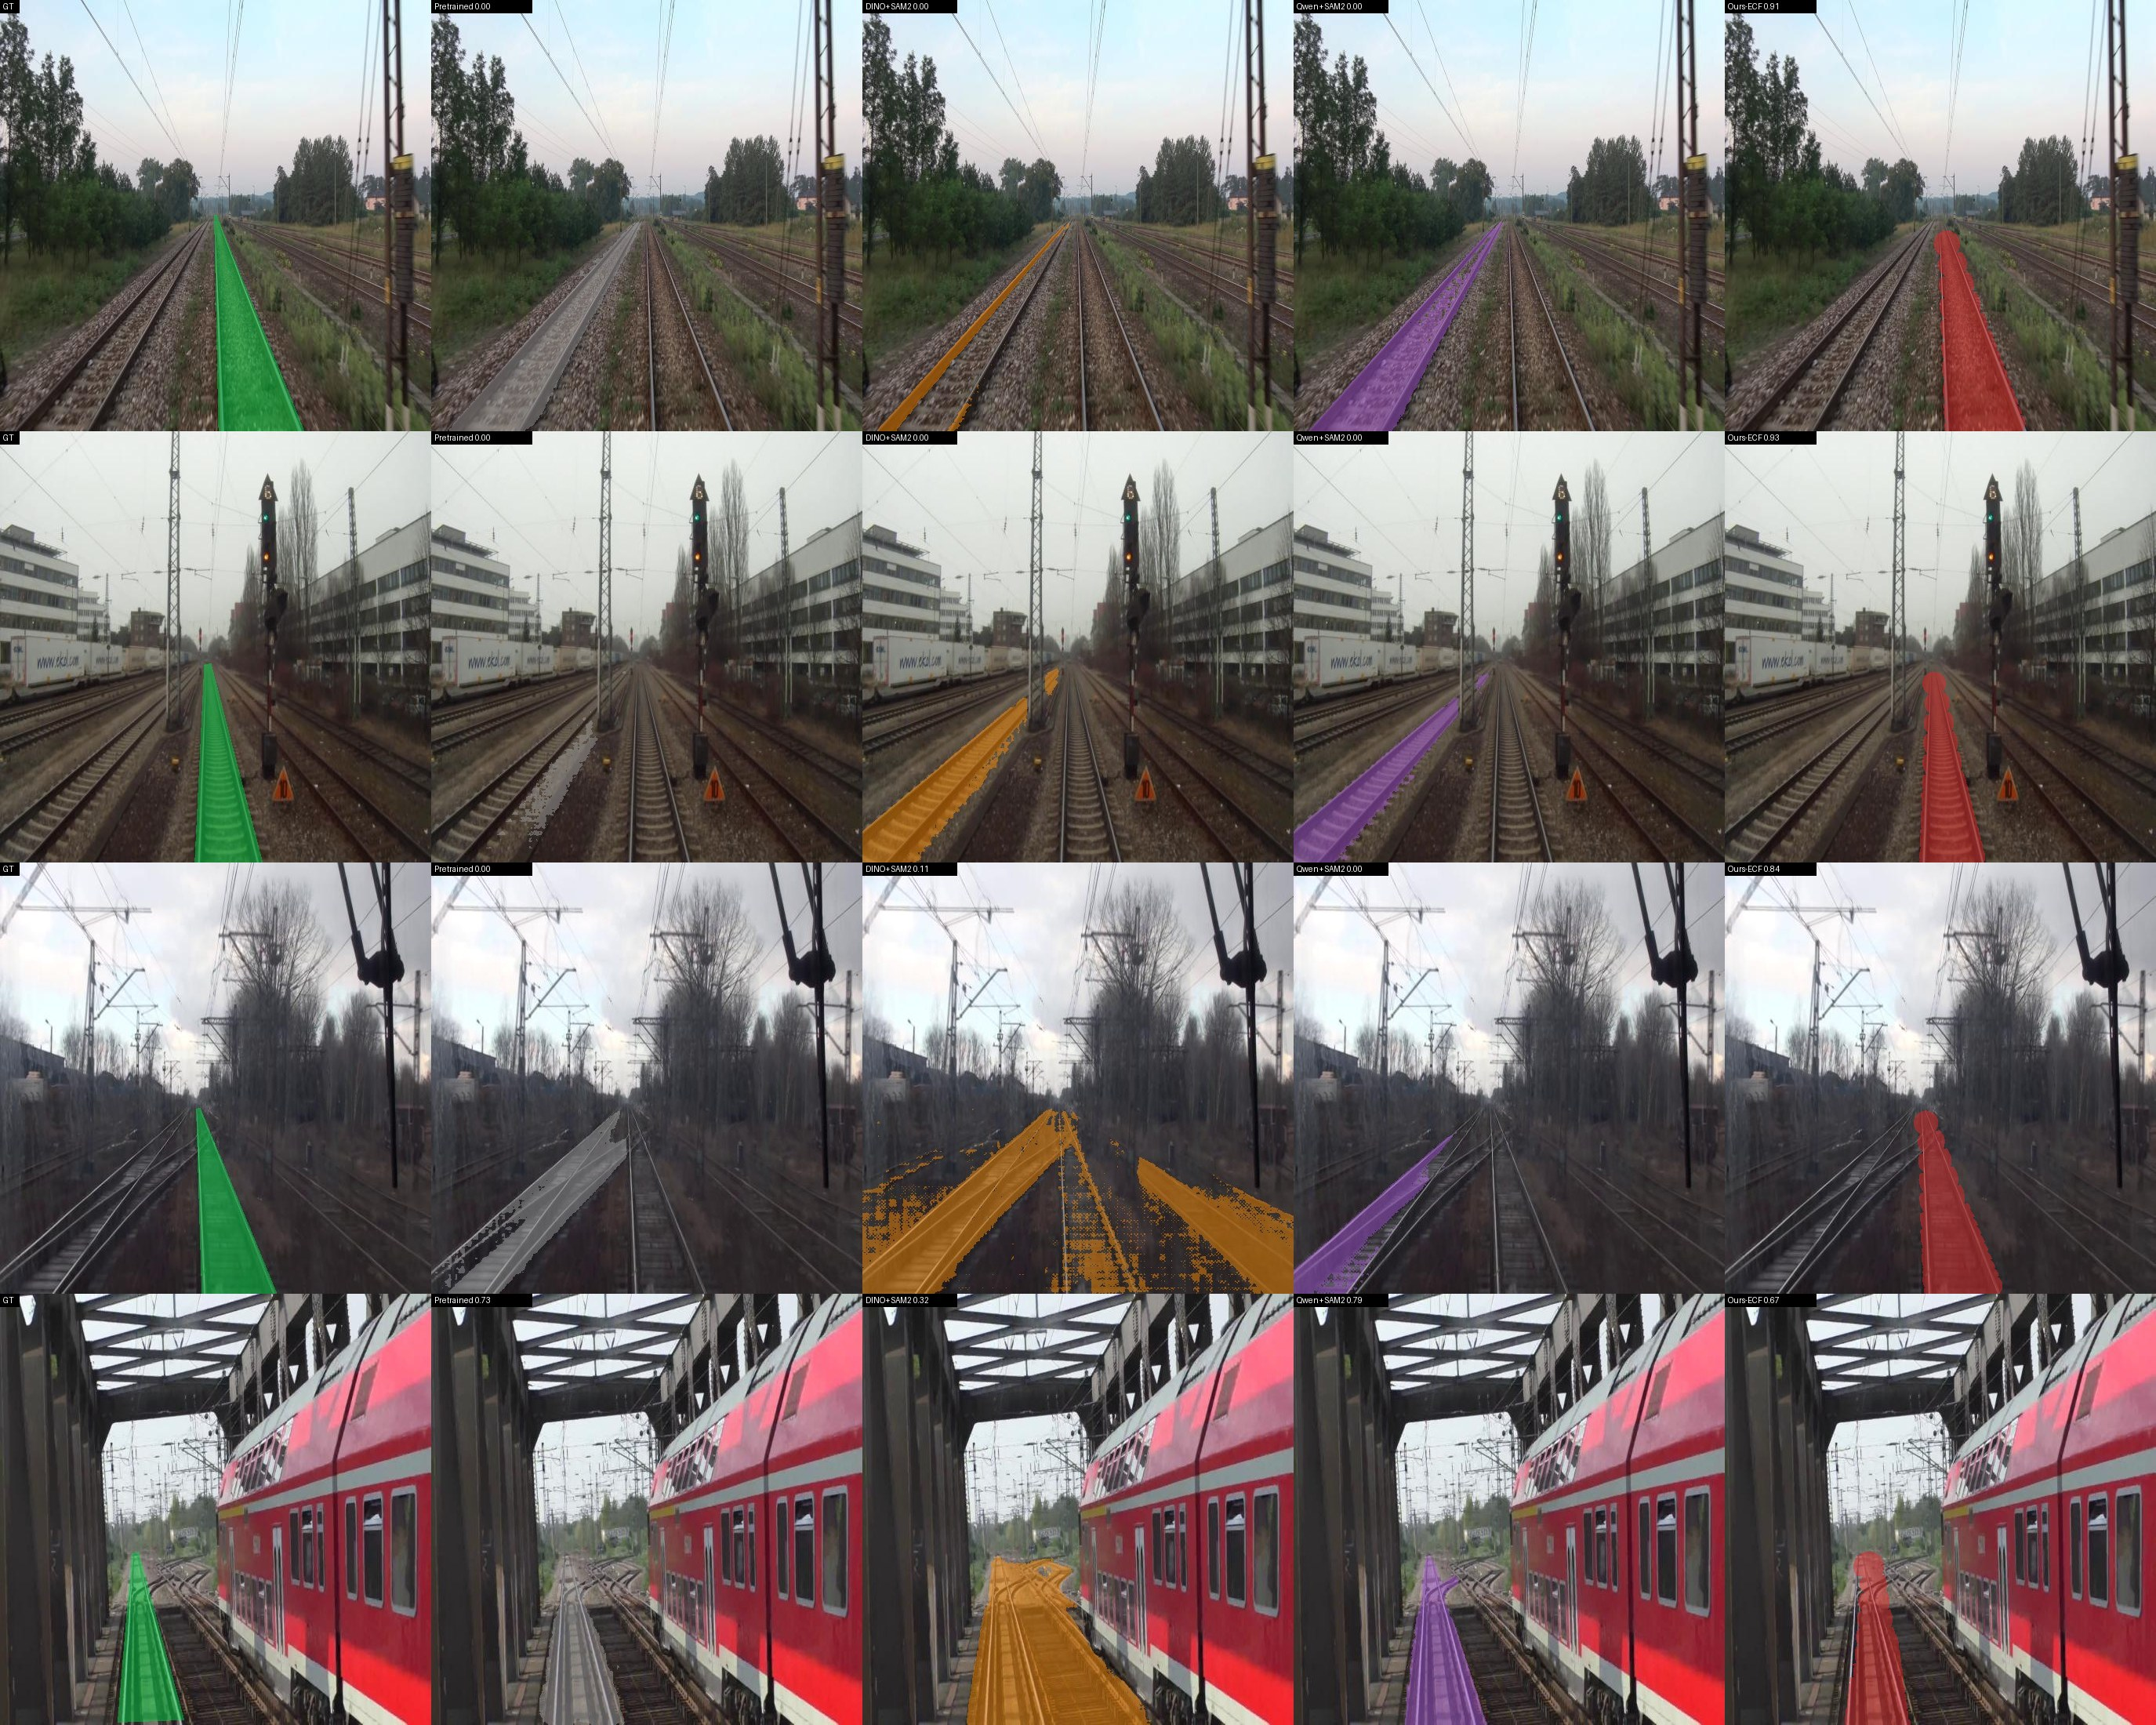
\includegraphics[width=\textwidth]{figures/fig1_qual.jpg}%
}{\fbox{\parbox{0.95\textwidth}{\centering\vspace{16mm}Qualitative panel pending.\vspace{16mm}}}}
\caption{Qualitative comparison on FIRC test (fp32). Columns: GT, pretrained Sa2VA, GroundingDINO+SAM2, Qwen2.5-VL-7B+SAM2, and our ECF-native rasterization. Panel labels give the per-image IoU of that column (two decimals). Panel labels come from the same evaluation runs as Table~\ref{tab:main}, so the figure and the table cannot disagree. In rows 1--3 both detector pipelines return no usable mask (0.00) or a small spurious one (0.11) on the ordinal caption, while ECF recovers a vanishing-point-aligned rail mask. Row 4 shows why a table of means alone is not enough: Qwen2.5-VL (0.79) and pretrained Sa2VA (0.73) do produce high-IoU masks, but on the \emph{wrong} rail: the target-selection failure that a mean score hides, and the failure mode ECF is built to avoid.}
\label{fig:qual}
\end{figure*}


\subsection{The rasterization loop is not optional}
\label{sec:ablate}

Table~\ref{tab:ablate} isolates the two falsifiers of the carrier claim; they are the A1/A2 panels of Figure~\ref{fig:framework}.
A1 doubles as the \emph{matched-training control} for Table~\ref{tab:main}: it reuses the trained LoRA and ParamHead of the main row and changes only the mask carrier, so any gap it shows is attributable to the carrier rather than to the mere presence of fine-tuning, and Table~\ref{tab:diag} shows the same falsifiers plus the width-profile limitation, one row per mechanism.

\paragraph{A1: same weights, SAM2 decode.}
We keep the ECF LoRA and ParamHead and instead route the \Seg{} embedding through SAM2, as a standard Sa2VA mask.
gIoU falls to 2.43, \PrAt{0.5} to 0.96 and \PrAt{0.7} to 0.0; TinyMaskRate (predicted mask under $0.1\%$ of the image area) is 30.29\%.
The embeddings that produce a corridor under $\cR$ are \emph{not} valid SAM2 prompts: this is the empirical counterpart of DeSa2VA's observation that extra signal into an entangled SAM2 pathway is not free, since here the extra signal is geometric and SAM2, as trained, does not read it.
It is also what rules out the trivial reading of Table~\ref{tab:main}, namely that ``fine-tuning simply helps'', because fine-tuning the same backbone and head with our recipe and then decoding with the original SAM2 carrier does not recover the gain.

\paragraph{A2: train without raster mask loss.}
An architecture-identical ECF model trained with $\lambda_{\mathrm{mask}}{=}0$ (parameter loss only; same orig$\cup$hflip schedule) reaches gIoU 69.31, \PrAt{0.5} 94.71, and \PrAt{0.7} \textbf{54.81}.
The head still emits a corridor-shaped region that often crosses IoU 0.5, but its high-IoU rate falls sharply: \PrAt{0.7} drops from 87.98 to 54.81, and pixel supervision through $\cR$ is the term that delivers \PrAt{0.7}---33.2 points above the no-mask-loss arm; $\phih^{gt}$ alone is not a substitute.

\begin{table}[t]
\centering
\small
\setlength{\tabcolsep}{3pt}
\caption{Carrier ablations on FIRC test ($n{=}208$, fp32). Row 1 is the main trained model. A1 reuses those trained LoRA/ParamHead weights with the SAM2 decoder and is the matched-training control for Table~\ref{tab:main}. A2 is an architecture-identical retrain with $\lambda_{\mathrm{mask}}{=}0$ on the same orig$\cup$hflip schedule.}
\label{tab:ablate}
\begin{tabularx}{\columnwidth}{@{}Ycccc@{}}
\toprule
Setting & \gIou & \PrAt{0.5} & \PrAt{0.7} & SegRate \\
\midrule
\textbf{ECF-native $\cR$} & \textbf{80.67} & \textbf{97.6} & \textbf{87.98} & 100.0 \\
A1: same weights $\to$ SAM2 & 2.43 & 0.96 & 0.0 & 100.0 \\
A2: $\lambda_{\mathrm{mask}}{=}0$ retrain & 69.31 & 94.71 & 54.81 & 100.0 \\
\bottomrule
\end{tabularx}
\end{table}

On the main run, 203/208 frames reach IoU ${\ge}0.5$ and 183/208 reach IoU ${\ge}0.7$; SegRate is 100\%, so every frame receives a mask.
Residual errors are geometric (thin far-field, boundary jitter), not detector-style empty masks, consistent with Figure~\ref{fig:qual}, and Figure~\ref{fig:ph_ecf_teaser} shows the same carrier over four ego-view rail settings.
On the same frames, the off-the-shelf reference systems fail in two different ways.
On the ordinal captions their masks are absent or negligible (Figure~\ref{fig:qual}, rows 1--3: 0.00 for both pipelines, and 0.11 for GroundingDINO+SAM2 in one case), so the mean in Table~\ref{tab:main} understates how rarely they solve the task at all; on the harder frame of row 4 they do return confident masks (Qwen2.5-VL at 0.79 and pretrained Sa2VA at 0.73) but on a different rail than the one the caption names.
A mean over gIoU cannot always separate ``found the referred rail'' from ``found a rail'': in row 4, the masks are confident yet land on the wrong rail, a target-selection failure under language rather than a mask-quality one.

Figure~\ref{fig:display} turns to the complementary diagnostic question of whether the $20$-D carrier can represent the referred corridor at all, across the shapes that occur in this split.
Each column shows one test frame with its ground-truth rail and the field reconstructed back to a mask, and each chip reports the \emph{reconstruction} IoU of that label-derived field against the ground-truth mask; it is a property of the carrier, not a model accuracy.
Corridors span the multi-rail ordinal case, the widest near-field in the split ($0.56$), and an occluded platform edge ($0.86$); over the $208$ test frames the reconstruction median is $0.891$ (supplementary material, Section~D).
Where the carrier is weakest, namely thin far-field and boundary jitter, is also where our residual error concentrates, which is the geometric failure mode claimed in Section~\ref{sec:ablate}.

\begin{figure*}[t]
\centering
\IfFileExists{figures/fig5_rail_qual.png}{%
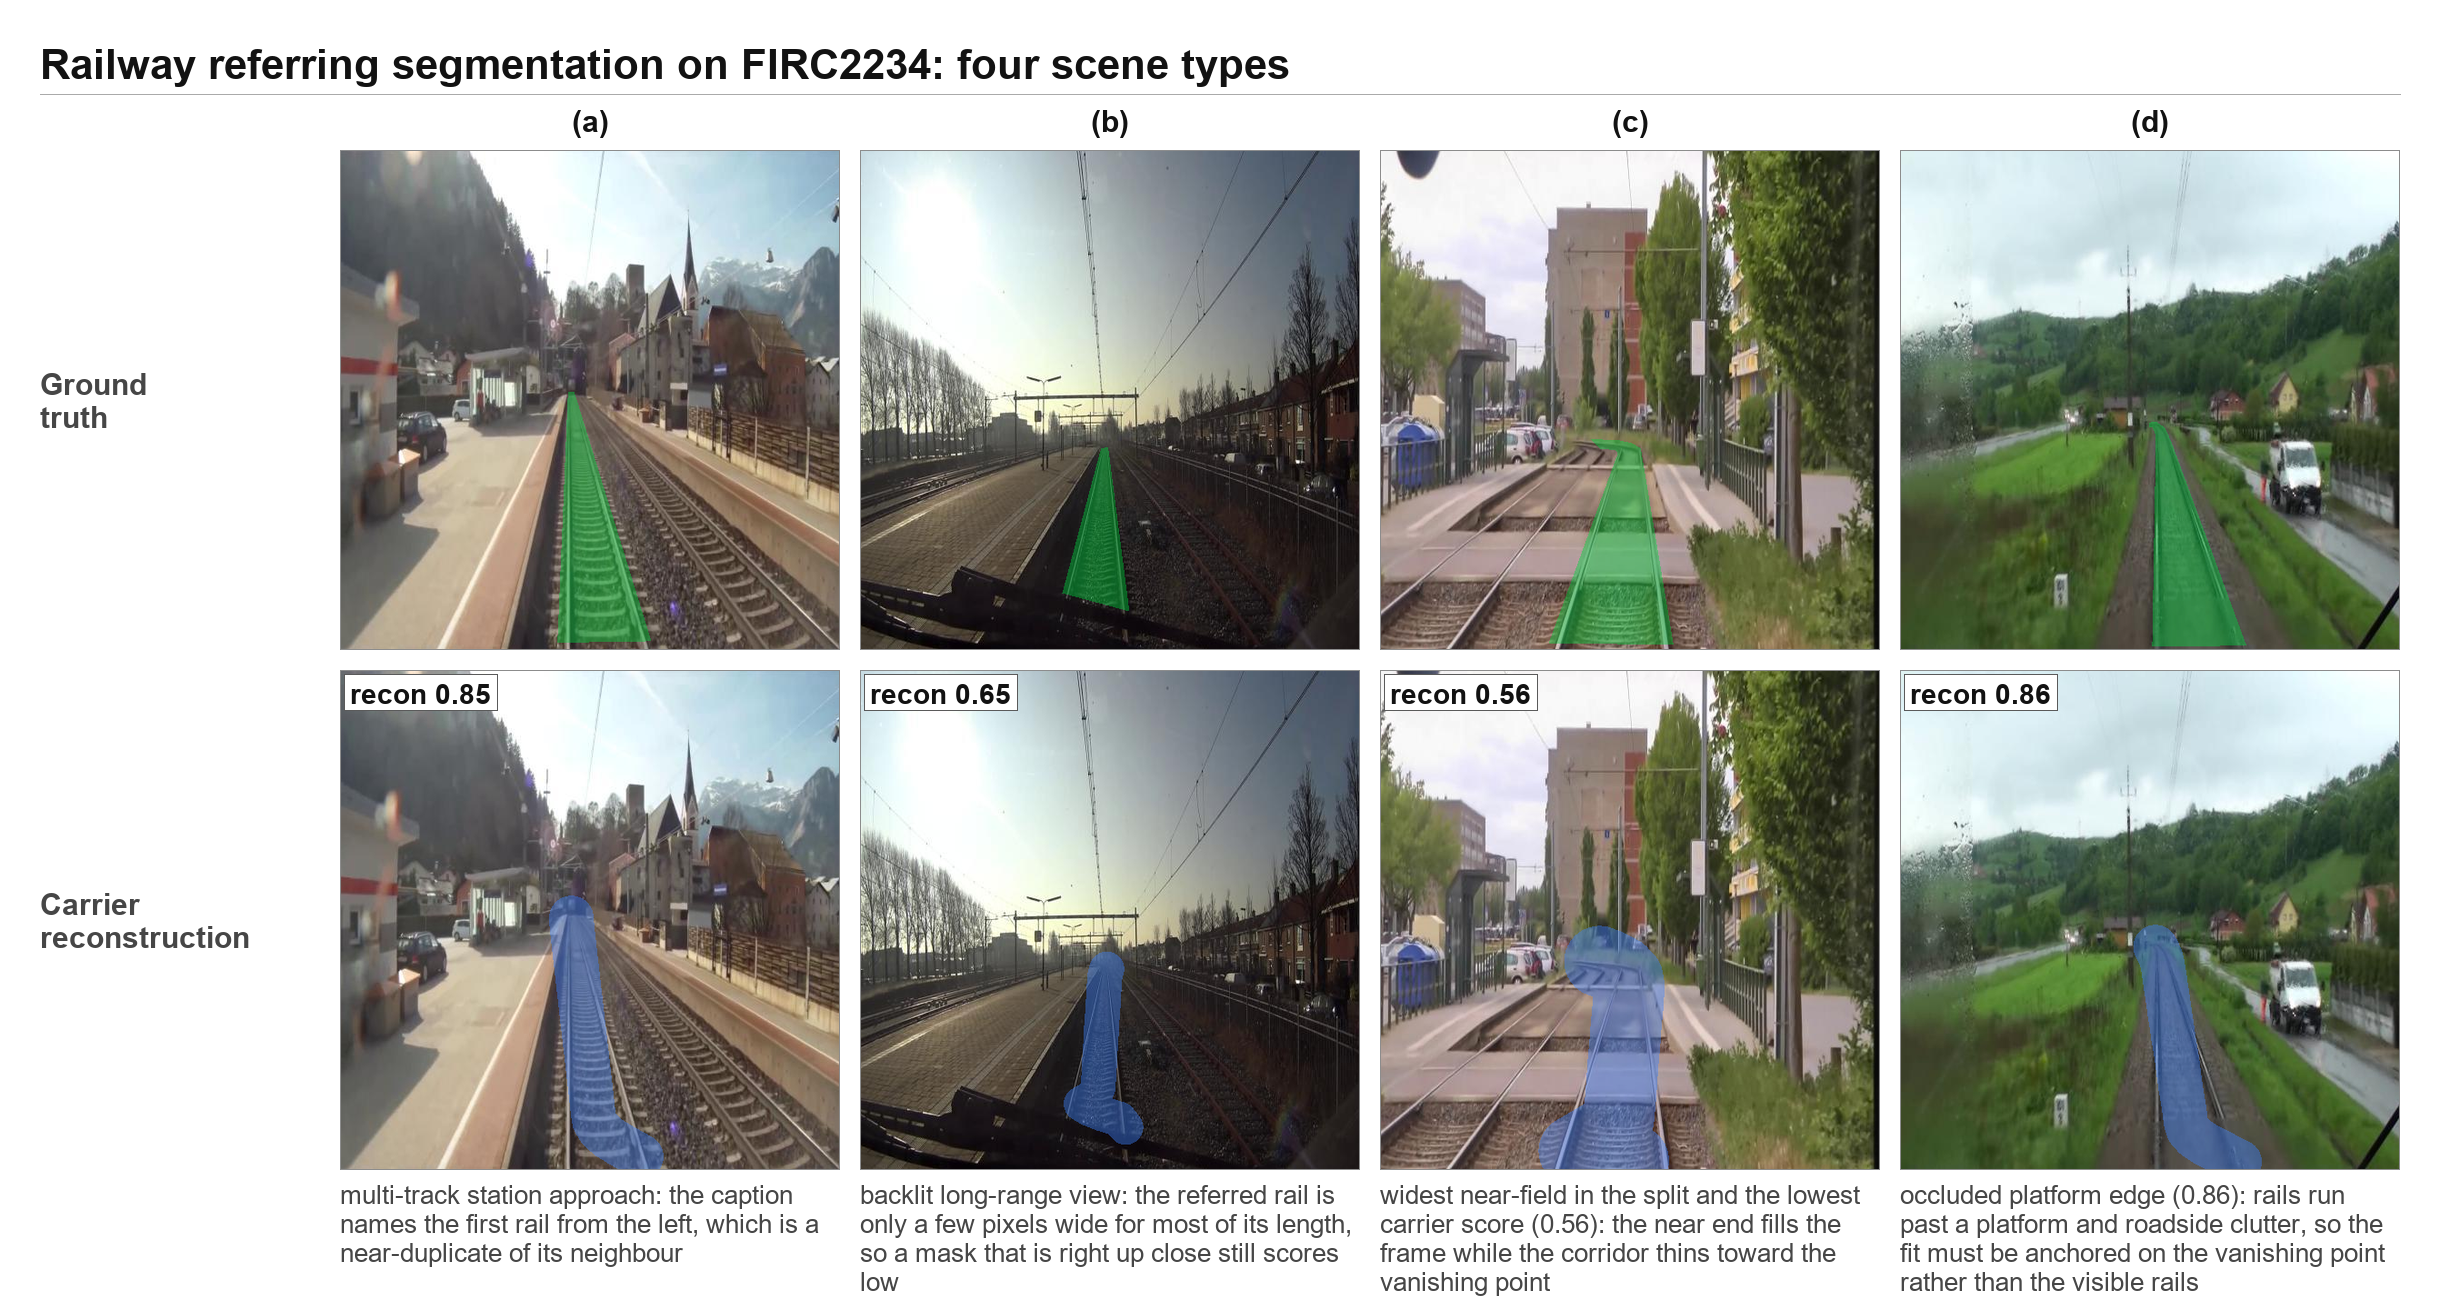
\includegraphics[width=\textwidth]{figures/fig5_rail_qual.png}%
}{%
\fbox{\parbox{0.95\textwidth}{\centering\vspace{14mm}Railway qualitative panel omitted in this build.\vspace{14mm}}}%
}%
\caption{What the carrier has to cover (FIRC2234 test, fp32 protocol).
Rows: the ground-truth referred rail and the reconstruction of the label-derived corridor carrier, both drawn as a translucent tint over the rails so the \emph{which rail} question stays visible.
Columns: one scene per challenge, labeled (a)--(d) as in the railway-segmentation literature, chosen to span the split.
(a)~a multi-track station approach, where the caption's ``first from left'' must be separated from near-duplicate neighbors ($0.85$);
(b)~a backlit long-range view, where the referred rail spans only a few pixels over most of its length ($0.65$);
(c)~the widest near-field frame in the split, where the near end fills the frame while the corridor thins toward the vanishing point ($0.56$);
(d)~an occluded platform edge, where the fit must be anchored on the vanishing point rather than the visible rails ($0.86$).
Chips give the per-frame \emph{recon IoU}, the reconstruction of the label-derived field against the ground-truth mask (median $0.891$ over $n{=}208$).
It measures the \emph{label} under the non-learned label-QA renderer of the supplementary material (Section~D), not the differentiable $\cR$ used in training, and is not comparable to Table~\ref{tab:main}.
Tiles are rendered from the dataset annotations and the corridor-label records; no model output enters this figure.
The panel is shared with the companion submission by the same authors and has not appeared elsewhere.}
\label{fig:display}
\end{figure*}

% ---------------------------------------------------------------------------
% [TABLE] carrier diagnostics -- converted from the former figure ecf_analysis_redraw.png
% ---------------------------------------------------------------------------
\begin{table}[t]
\centering
\small
\setlength{\tabcolsep}{3pt}
\caption{Three diagnostics that isolate what the loop removes (FIRC test, fp32, $n{=}208$). Rows (a)/(b) are the two falsifiers of Table~\ref{tab:ablate}; row (c) records the width-profile limitation: the rasterizer consumes only the per-side mean of the stored width samples, so a width profile along the corridor is deliberately not represented.}
\label{tab:diag}
\begin{tabularx}{\columnwidth}{@{}YYY@{}}
\toprule
Diagnostic & Setting & Result \\
\midrule
(a) raster carrier, not SAM2 decode & same trained $h$, SAM2 decode & $80.67 \to 2.43$ \gIou \\
(b) mask loss off & $\lambda_{\mathrm{mask}}{=}0$ retrain & $69.31$ \gIou, $\PrAt{0.7}{=}54.81$ \\
(c) width profile & per-side mean only & envelope not represented \\
\bottomrule
\end{tabularx}
\end{table}

Table~\ref{tab:diag} isolates, one row at a time, the elements that the loop removes.


\subsection{Eval-only transfer and harder captions}
\label{sec:transfer}

The FIRC checkpoint is frozen, and Table~\ref{tab:transfer} reports two additional single-rail fill-band protocols, each with its own off-the-shelf reference set (never copied from Table~\ref{tab:main}).
RailSem19-EgoPair keeps frames with exactly one polyline pair ($n{=}300$ test) and RailBench 1L1R keeps frames with exactly one left and one right rail polyline ($n{=}260$); neither set is used for training, and ECF keeps the best gIoU on each protocol (66.93 vs.\ 41.90 on EgoPair; 54.21 vs.\ 46.35 on RailBench).

\begin{table*}[t]
\centering
\small
\setlength{\tabcolsep}{4pt}
\caption{Eval-only transfer. Not mixed into Table~\ref{tab:main}. Caption template matches FIRC. Reference rows are off-the-shelf systems; ECF rows reuse the frozen FIRC checkpoint with no further training (EgoPair $n{=}300$; RailBench 1L1R $n{=}260$).}
\label{tab:transfer}
\begin{tabularx}{\textwidth}{@{}Ycccc@{}}
\toprule
Protocol / method & \gIou & \PrAt{0.5} & \PrAt{0.7} & SegRate \\
\midrule
EgoPair, pretrained Sa2VA & 12.48 & 8.67 & 5.67 & 100.0 \\
EgoPair, GroundingDINO+SAM2 & 41.90 & 41.33 & 33.67 & 99.3 \\
EgoPair, Qwen2.5-VL-7B+SAM2 & 38.93 & 42.67 & 31.33 & 100.0 \\
\textbf{EgoPair, ECF (FIRC ckpt)} & \textbf{66.93} & \textbf{94.00} & \textbf{45.67} & 100.0 \\
\midrule
RailBench 1L1R, pretrained Sa2VA & 16.46 & 16.92 & 9.23 & 100.0 \\
RailBench 1L1R, GroundingDINO+SAM2 & 46.35 & 49.62 & 38.08 & 99.2 \\
RailBench 1L1R, Qwen2.5-VL-7B+SAM2 & 7.07 & 7.31 & 6.15 & 100.0 \\
\textbf{RailBench 1L1R, ECF (FIRC ckpt)} & \textbf{54.21} & \textbf{70.38} & \textbf{31.92} & 100.0 \\
\bottomrule
\end{tabularx}
\end{table*}

\paragraph{On linguistic control.}
A natural concern about a single-rail set is that the model may ignore the caption and segment the only rail present.
FIRC2234 cannot settle this: every test frame carries the same caption string, and a caption that names a non-existent neighboring branch cannot be scored as an instance switch (Table~\ref{tab:data}).
What we can show is insensitivity to a same-target paraphrase: with harder rephrasings of the \emph{same} target (same masks), ECF stays at 80.97 gIoU (Table~\ref{tab:hardref}), within 0.3 points of the 80.67 obtained with the original caption.
A caption-swap probe, which feeds one frame the caption of a \emph{different} target and checks that the predicted mask moves, requires multi-rail frames with distinct per-rail captions, which FIRC2234 does not contain; we therefore flag it as the most important missing experiment for a linguistic-control claim (Section~\ref{sec:conclusion}) rather than over-read the paraphrase table.

\begin{table}[t]
\centering
\small
\setlength{\tabcolsep}{3pt}
\caption{Same FIRC test masks, harder same-target paraphrases ($n{=}208$, fp32). This is a robustness probe, not a linguistic-sensitivity test; see the text.}
\label{tab:hardref}
\begin{tabularx}{\columnwidth}{@{}Ycccc@{}}
\toprule
Caption / method & \gIou & \PrAt{0.5} & \PrAt{0.7} & SegRate \\
\midrule
Hard-ref, pretrained Sa2VA & 4.80 & 5.29 & 2.88 & 100.0 \\
\textbf{Hard-ref, ECF} & \textbf{80.97} & \textbf{97.60} & \textbf{86.54} & 100.0 \\
\bottomrule
\end{tabularx}
\end{table}

\section{Discussion: two treatments of a sparse \Seg{} token}
\label{sec:discussion}

The empirical core is that a 20-D corridor can be rasterized, and that the sparse \Seg{} prompt DeSa2VA locates \emph{inside} the token can be addressed from the \emph{decoder} side, not only by splitting the token.

\paragraph{Carrier replacement vs.\ DeSa2VA's architectural decoupling.}
DeSa2VA \citep{dang2025desa2va} splits a Sa2VA hidden state into text and visual streams \emph{before} SAM2, because a single \Seg{} token cannot carry both semantics and a dense visual prompt.
ECF never splits that state and never asks SAM2 to become a better prompt reader; it lets the entangled token bind a caption to an object---what language models already do---and writes the dense spatial structure as $\phih$.
Two independent observations support this reading.
First, A1: the same $h$ that rasterizes a rail is a useless SAM2 prompt (2.43 gIoU), so the information is in the ParamHead$+\cR$ path, not in some latent SAM2-compatible embedding.
Second, DeSa2VA's own ablation shows that extra text-derived mask supervision into an entangled \Seg{} pathway hurts Sa2VA (RefCOCO 78.9$\to$73.4 without decoupling).
We do not feed extra text into SAM2; we stop feeding $h$ into SAM2 on the evaluated path, and we are not claiming to reproduce DeSa2VA's RefCOCO gains, only that the sparse-prompt diagnosis has a decoder-side, geometric treatment as well as an encoder-side one.

\paragraph{Low-dimensional corridors vs.\ free masks.}
Parametric lane heads \citep{tabelini2021polylanenet,feng2022bezierlanenet} already treat ego-view rails as polylines.
What is new here is the \emph{binding}: the polyline is the meaning of a referring \Seg{} token inside an MLLM, trained with a raster closed loop so that language gradients and geometry gradients share $h$.
Figure~\ref{fig:framework} draws this forward path (Section~\ref{sec:method}), and Figure~\ref{fig:display} shows the shapes the field must cover across this split.
A2 shows the loop is load-bearing: without $\mathcal{L}_{\mathrm{mask}}$, \PrAt{0.7} drops to 54.81 even though a parameter loss is present.

\paragraph{Carrier versus backbone.}
The control that isolates the carrier is internal to our system rather than external: A1 reuses the same trained LoRA and ParamHead and changes only where the mask comes from, giving 2.43 versus 80.67 gIoU.
That already undercuts the trivial reading that the masks come from the language backbone.
The carrier claim itself stands on A1 and on the failure mode of Figure~\ref{fig:qual} row 4, where high-IoU masks land on the wrong rail: on this target, decoder strength by itself did not deliver target selection; changing the carrier did.

\paragraph{What this paper does and does not replace.}
The two treatments are not substitutes: decoupling improves the encoder-side prompt that a generalist SAM2 receives, while ECF assumes a corridor target and changes the decoder.
We read them as alternatives for different target classes rather than as a refutation of either.

\section{Conclusion and Limitations}
\label{sec:conclusion}

We presented Ego-Corridor Fields for Sa2VA-style referring segmentation: a 20-D corridor parameterization predicted from the \Seg{} token and rasterized differentiably, with SAM2 bypassed.
The design is a decoder-side alternative to DeSa2VA's architectural decoupling \citep{dang2025desa2va}: a treatment for corridor-shaped targets, complementary to their encoder-side one and to parametric lane heads \citep{tabelini2021polylanenet,feng2022bezierlanenet}.
On FIRC2234 test (original$\cup$hflip train), ECF-native decoding reaches gIoU 80.67 and outperforms the off-the-shelf reference set by 2.9--3.2$\times$ (and the pretrained model by 5.6$\times$) under the same protocol, winning 89.4--93.8\% of pairwise comparisons.
The matched-training control A1 shows where the gain comes from: the identical trained backbone and head decoded by SAM2 collapse, so the improvement is attributable to the carrier rather than to fine-tuning alone.
A1 and A2 further indicate that the raster loop is load-bearing: SAM2, as trained, does not read ECF embeddings (2.43 gIoU), and parameter supervision without mask loss leaves \PrAt{0.7} at 54.81, 33.2 points below the full model (87.98).
The same checkpoint transfers eval-only to EgoPair (66.93) and RailBench 1L1R (54.21).

\textbf{Limitations.}
(1)~ECF assumes a corridor-shaped target; it is not a general RES decoder for compact instances.
(2)~The carrier-versus-fine-tuning separation rests on A1, which reuses our trained weights and changes only the decoder; a Sa2VA fine-tuned with its native mask loss on FIRC is not evaluated.
(3)~FIRC2234 carries a single caption template, so we can show robustness to paraphrase but not \emph{sensitivity} to a swapped target caption; a caption-swap probe needs multi-rail frames and remains the most important missing experiment.
(4)~Topology logits are reserved but unused as a fork verifier; multi-rail disambiguation is future work.
(5)~Transfer sets are eval-only fill-bands with a shared caption template, not independently annotated referring corpora.
(6)~We do not re-implement DeSa2VA or parametric lane detectors on FIRC; the connection is mechanistic, not a head-to-head comparison.
(7)~A weak width-monotonicity term is included but not claimed; a later, heavier physics recipe failed to help and is not a main result.
(8)~Strict \PrAt{0.7} (87.98) sits 9.6 points below \PrAt{0.5} (97.6); residual errors concentrate on far-field thin structure.
(9)~All main results come from a single training run on a single backbone (InternVL3-2B Sa2VA weights); run-to-run variance is not reported and the detector rows use a fixed leftmost-box rule (alternatives not swept).

\textbf{Future work.}
We are pursuing five directions: (i)~a caption-swap probe on multi-rail frames, for linguistic sensitivity rather than paraphrase robustness; (ii)~a Rail-Path Verifier on the topology logits for forks; (iii)~DeSa2VA-style split heads so that $\phih$ comes from a visual stream, not an entangled $h$; (iv)~dropping SAM2 from the training graph entirely; and (v)~video rails, where a corridor field has a natural temporal smoothness prior.
Code, checkpoints, and evaluation scripts will be released upon acceptance under the source datasets' licenses, and the authors declare no competing interests.


% Appendix A was moved out of the manuscript into the standalone supplementary
% document (main_supplementary.tex + sections/A_appendix_supp.tex) to bring the
% Transactions Paper inside the IEEE TCSVT 14-page ceiling.  The content was moved,
% not deleted: sections/A_appendix.tex is kept in the source tree as the record.

% Flush every pending float before the bibliography so that no figure is
% emitted after the reference list (figure-heavy, full-width floats).
\clearpage
\bibliographystyle{IEEEtran}
\bibliography{references}

\end{document}
